\documentclass[12pt]{article}
\usepackage[T2A]{fontenc}
\usepackage[utf8]{inputenc}
\usepackage[russian]{babel}
\usepackage{ dsfont }
\usepackage{amsmath,amssymb}
\usepackage{amsthm}
\usepackage{mathtools}
\usepackage{tikz}
\usepackage{graphicx}
\usepackage{gensymb}
\usepackage{indentfirst}
\usepackage{textcomp}
%for subfigures
\usepackage{caption}
\usepackage{subcaption}

%\usepackage{biblatex}
\usepackage{csquotes}
\usetikzlibrary{arrows.meta}


% \usepackage[bottom=1in,top=0.8in]{geometry}
\textheight=24cm % высота текста
\textwidth=16cm % ширина текста
\oddsidemargin=0pt % отступ от левого края
\topmargin=-1.5cm % отступ от верхнего края
\parindent=24pt % абзацный отступ
\parskip=0pt % интервал между абзацами
\tolerance=2000 % терпимость к "жидким" строкам
\flushbottom % выравнивание высоты страниц


\usepackage{hyperref}
\hypersetup{
    colorlinks=true,
    allcolors=blue
}

\usepackage{xcolor}
% \usepackage{colortbl}

	
\usepackage{algorithm}
\usepackage{algpseudocode}
\floatname{algorithm}{Алгоритм}
\algnewcommand{\And}{\textbf{ and }}
\algnewcommand{\Or}{\textbf{ or }}

\usepackage{tikz}
\usetikzlibrary{arrows,automata,positioning}


\bibliographystyle{gost-numeric.bbx}
\usepackage[parentracker=true,
backend=biber,
hyperref=true,
bibencoding=utf8,
style=numeric-comp,
language=auto,
autolang=other,
citestyle=gost-numeric,
defernumbers=true,
bibstyle=gost-numeric,
sorting=none,
]{biblatex}
\addbibresource{bib.bib}

\graphicspath{ {pics} }

\def \deg {\degree}
\def \N {\mathbb{N}}
\def \R {\mathbb{R}}
\def \K {\mathcal{K}}
\def \I {\mathcal{I}}

\def \eps {\varepsilon}
\DeclareMathOperator{\sign}{sign}
\DeclareMathOperator*{\E}{\mathbb{E}}

\newcommand{\defeq}{\vcentcolon=}
\newcommand{\eqdef}{=\vcentcolon}

\newcommand{\norm}[1]{\left\lVert#1\right\rVert}
\newcommand {\Def}[0]       {\textbf{Определение.} }

\newtheorem {Statement}{Утверждение}

\begin{document}

\newpage

\section*{Введение}
\addcontentsline{toc}{section}{\protect\numberline{}Введение}

\paragraph{Актуальность темы.}
Магистерская работа посвящена исследованию задачи распределённого управления изолированной энерго(электро)системой.
Для поддержания устойчивости энергосистемы и эффективности её работы в изменяющихся условиях (например, изменение уровня потребления электроэнергии) необходимо в реальном времени решать задачу выбора мощности генерации (\textit{уставок}) для каждой электростанции.
Поскольку электрическая сеть~--- физически связанная система, уставки для генерирующих электростанций должны согласовываться между собой.

Традиционно (например, в Единой энергетической системе России \cite{eesfreqpower}), эта задача решается централизованным/иерархическим способом: диспетчерские центры собирают информацию о состоянии энергосистемы и выдают уставки генерирующим станциям.
В современных энергетических системах с внедрением возобновляемых источников энергии (ВИЭ) увеличивается количество генерирующих устройств, генерация распределяется по потребительской сети.
Домашние хозяйства с установленными солнечными и ветроэнергетическими станциями могут в разные моменты времени выступать как потребители, или как производители электроэнергии.
Увеличение количества генераторов и динамически меняющаяся топология сети создаёт проблемы для централизованных систем управления: проходящие через один узел потоки данных перегружают каналы передачи информации, вычислительная сложность задачи может превышать аппаратные возможности одного устройства.
С распространением дешёвых и производительных одноплатных компьютеров построение надёжной (устойчивой к отказу одного узла) и быстрой системы управления на основе децентрализованного подхода может стать более эффективным решением, чем реализация традиционной централизованной схемы.

Другая особенность современных энергосистем, связанная с внедрением ВИЭ~--- влияние внешних условий на генерацию электроэнергии.
Суточные осцилляции солнечной активности и стохастическая природа ветра приводят к рассогласованию между спросом и предложением и возникновению избыточной электроэнергии, особенно в изолированных системах с большой долей ВИЭ.
Для решения этой проблемы приходится использовать накопители энергии и/или подстраивать график потребления электроэнергии под профиль генерации ВИЭ.

Учет этих особенностей приводит к тому, что постановка задачи управления энергосистемой существенно отличается от традиционной.

В России применение технологий микрогридов и ВИЭ особенно актуально в северных районах, изолированных от единой энергосети.
Используемые в изолированных поселениях на данный момент дизельные электростанции экологически и экономически неэффективны~--- экономически обоснованные тарифы на электроэнергию могут быть в десятки раз выше, чем в присоединённых к единой энергосети областях \cite[15]{ancenter2017tarifes}.
Так, в 2019--2021 годах Инжиниринговый центр «Арктическая Автономная Энергетика» МФТИ выполнял проект модернизации действующей дизельной генерации с введением в эксплуатацию ветроэнергетической установки в энергоизолированном посёлке Лаборовая Приуральского района Ямало-Ненецкого автономного округа.
Математического и программное обеспечение этого проекта~--- одна из целей выполнения данной работы.

В данный момент темы распределённых информационных систем и распределённых алгоритмов оптимизации характеризуются высокой научной активностью.
Это же свойственно и теме \textit{микрогридов}~--- единиц энергетической сети с распределённой генерацией \cite{lasseter2002microgrids}.
% краткий обзор?
Поэтому имеется очень много результатов о распределённых системах оптимизации и обосновании оптимизационных постановок задач управления изолированными энергетическими системами, однако, насколько нам известно, комплексного описания распределённой системы управления для изолированной энергосистемы с различными типами генераторных и аккумулирующих устройств и преобладанием тепловой нагрузки (что характерно для объектов, расположенных на северных территориях) в литературе нет (конечно, надежда на то, что какой-нибудь индус не опубликовал аналогичную статью лет 10 назад довольна слаба, но зачем её искать и портить себе настроение). 



This is not surprising as OPF has been
shown in [25], [39], and [40] to be NP-hard in general. \cite{lehmann2015ac}

 
 
 
 \paragraph{Цель работы.}
 Целью работы является разработка децентрализованной системы управления изолированной гетерогенной по типу систем генерации и накопления энергии энергосистемой, учитывающей преобладающий характер тепловой нагрузки для применения в проектируемых и перспективных объектах арктической зоны.
 
 \paragraph{Методы исследования.}
 Для достижения поставленных целей используется аппарат теории оптимизации.
 Программная реализация выполнена на языке Python3.
 Проверка работы системы осуществлена на тестовом стенде Инжинирингового центра «Арктическая Автономная Энергетика» МФТИ в составе кластера одноплатных компьютеров Raspbery PI и Tinkerboard, на которых размещена система управления, и программно-аппаратного комплекса физического моделирования режима реального времени RTDS.
 
 
 
 \paragraph{Основные положения, выносимые на защиту.}
 \begin{enumerate}
   \item Децентрализованная система управления изолированным микрогридом, разработанная с учетом особенностей арктического применения.
   \item Методы анализа критериев эффективности системы управления, относящихся к использованию систем накопления энергии.
 \end{enumerate}
 
 
 
 \paragraph{Научная новизна.}
Получена верхняя оценка эффективности системы накопления энергии, в которой одно устройство  работает в астатическом по частоте и напряжению режиме, а остальные~--- в астатическом по мощности режиме.
Проведён анализ алгоритмов подсчёта циклов в кривых заряда-разряда устройств накопления энергии.
Дано комплексное описание принципов построения децентрализованной системы управления изолированным микрогридом с уклоном в применение в арктических условиях.
 
 
%  \paragraph{Теоретическая значимость.}
%  Данное исследование вносит существенный вклад в область согласования прогнозов иерархических временных рядов, связанный с разработкой нового подхода к согласованию прогнозов, который не имеет недостатков, присущих ранее разработанным методам, и, следовательно, имеет более широкую область применения.
 
 
 \paragraph{Практическая значимость.}
 Разработанная система отличается простотой, эффективностью и широким потенциалом применения в активно развивающейся области модернизации и введения в эксплуатацию новых арктических автономных систем энергоснабжения.
 
 
 \paragraph{Степень достоверности и апробация работы.}
 Достоверность результатов подтверждена математическими доказательствами и экспериментальной проверкой работы системы на детальной физической модели. 
 Результаты работы использовались в коммерческих проектах Инжинирингового центра «Арктическая Автономная Энергетика» МФТИ.
 
 
%  \paragraph{Публикации по теме.}
%  Основные результаты по теме магистерской работы изложены в изданиях из списка ВАК \cite{medvednikova2012algorithm, kuznetsov2012algorithm, medvednikova2013construction, stenina2014reconciliation, gazizullina2015forecasting, stenina2015reconciliation}, двух сборниках докладов конференций \cite{stenina2014mipt, stenina2015lomonosov} и других печатных изданиях \cite{medvednikova2012pca, Stenina2015ordinal}.
 
 
\newpage
\section{Централизованный подход}
Назначение верхнеуровневой системы управления микрогридом~--- экономически оптимальное распределение мощности между генерирующим и аккумулирующим оборудованием и нагрузкой (задачи \textit{unit commitment} или \textit{optimal dispatch}).

Из этой задачи отдельно можно выделить задачу управления режимом работы оборудования: часто приведение устройства в рабочий режим связано с затратами энергии и расходованием ресурса оборудования.
Например, запуск дизель-генератора требует его предварительного прогрева, а условия его эксплуатации не допускают частых включений-выключений из-за износа \cite{bleijs1993wear}, поэтому, будучи включен в отсутствии нагрузки, он будет вынужден работать некоторое время на холостом ходу.
Топливные элементы и электролизные установки так же требуют предварительного прогрева и времени для выхода на режим. 
Поэтому будем отдельно рассматривать \textit{задачу выбора уставок} мощности и задачу выбора режима работы оборудования~--- \textit{задачу планирования}.
%  \textit{откладываемой} нагрузкой, т. е. нагрузкой, удовлетворение которой может быть сдвинуто во времени, например, нагрузка на обогрев помещения 

Структура этого раздела следующая:
в начале мы сформулируем  задачу планирования (подразделы \ref{sec:system_definition}--\ref{sec:planning_math}),
и приведём результаты численных экспериментов (подраздел \ref{sec:planning_numeric}).
Затем покажем, что задача выбора уставок может быть сведена к практически такой же математической формулировке.
Завершает раздел обзор более продвинутых подходов к задаче планирования.
Результаты численных экспериментов будут приведены сразу для децентрализованной системы управления в разделе \ref{sec:decentralized}.

Цель этого раздела~---  введение наиболее простой модели, отражающей основные особенности изолированной энергосистемы, формулировка и имплементация простой системы управления в виде оптимизационной задачи и интерпретация полученных результатов.
Хотя возможно построение простых систем управления, имеющих вид цепочек условных операторов \cite{Aziz2019}, дизайн таких систем управления предполагает, что выполнены определённые соотношения между параметрами компонентов управляемой системы, поэтому они не универсальны и являются частными решениями универсальных оптимизационных задач управления энергосистемой.
Ещё одним плюсом описания системы управления в виде оптимизационной задачи является возможность добавления ограничений и учёта новых факторов без существенного изменения кода или даже в рамках одной математической формулировки.

Содержание этого раздела близко к содержанию статьи Barley, Winn \cite{Barley1996}, в которой проводится сравнительный анализ эвристических стратегий управления микрогридом. 
Общий подход к задаче, предложенный в статье Barley, Winn, используется в одном из наиболее популярных программных пакетов для оптимального дизайна микрогридов Homer Pro, часто применяемом для валидации результатов в научных работах \cite{Berendes2018, Aziz2019, Petersen2018, Olatomiwa2016}.

% \subsection{Постановка задачи}
% \label{sec:planning_problem}
\subsection{Описание компонентов физической системы}
\label{sec:system_definition}

Решается задача оптимального управления автономной энергетической системой.\\
Рассматриваемая система включает неконтроллируемый источник ``бесплатной'' возобновляемой энергии  (ветрогенератор или фотовольтаическая солнечная установка), дизель-генератор, накопитель энергии и постоянную неуправляемую нагрузку.
В качестве базового варианта накопителя энергии рассматривается литий-ионный электрохимический аккумулятор, ставший вариантом по-умолчанию для установки в микрогридах за счёт оптимального соотношения между мощностью и энергетической ёмкостью, хорошему ресурсу и способностью практически мгновенно изменять величину потребляемой/выдаваемой мощности.
С соответствующими допущениями написанное в этом разделе можно применить и к другим типам накопителей. 

Пренебрегая зависимостью интенсивности износа аккумуляторной батареи от глубины заряда/разряда и величины токов, считаем, что стоимость использования батареи определяется её капитальной стоимостью и ресурсом, равным количеству электрической энергии, которая может пройти через батарею до того, как батарею необходимо будет заменить.
Таким образом, стоимость использования батареи определяется по формуле \cite{bwc}:


\begin{equation}\label{f:cb}
c_b(P) \left[\frac{\$}{h} \right] = 
a_b \cdot P,
\end{equation}
\begin{equation}\label{f:ab}
a_b \left[ \frac{\$}{kW\cdot h} \right] =
\frac{\text{batteryPrice}}{\text{batteryCapacity} \cdot \text{batteryMaxCycles} 
\cdot \sqrt{\eta}} ,
\end{equation}
здесь batteryPrice~[\$]~--- капитальная стоимость батареи,\\
batteryCapacity~[$kW\cdot h$]~--- энергетическая ёмкость батареи,\\
batteryMaxCycles~--- число полных циклов заряда-разряда до замены батареи,\\
$\eta$~--- энергетический КПД цикла заряда-разряда.

    
Для включенного дизельного генератора зависимость расхода топлива от мощности:
\begin{equation}
 \text{fuelConsumption} (P) = \text{fuelIntercept} + \text{fuelSlope} \cdot P.
\end{equation}

Тогда стоимость использования дизель-генератора:

\begin{equation}\label{f:cg}
c_g(P) \left[\frac{\$}{h} \right] = b_g + a_g \cdot P,
\end{equation}


\begin{equation}\label{f:bg}
b_g \left[\frac{\$}{h} \right] = 
\text{fuelIntercept} \cdot \text{fuelCost} + \text{maintainanceCost} +
\frac{\text{gensetPrice}}{\text{gensetResource}},
\end{equation}

\begin{equation}\label{f:ag}
a_g \left[ \frac{\$}{kW\cdot h} \right] = 
\text{fuelSlope} \cdot \text{fuelCost}.
\end{equation}
Здесь maintainanceCost~[\$ / моточас]~--- стоимость обслуживания,\\ 
gensetPrice~[\$]~--- капитальная стоимость генераторной установки,\\
gensetResource~[моточас]~--- количество моточасов до замены.

Здесь предполагается, что ресурс дизель-генератора, в отличии от ресурса электрохимического аккумулятора, зависит от количества часов в работе, но не зависит от мощности.
Действительно, основной показатель надёжности, предоставляемый производителями дизель-генераторов~--- это время наработки на отказ   (ГОСТ Р 53176-2008). 
Кроме того, аналогичная электрохимическим накопителям модель деградации, в которой ресурс зависит от выработанной энергии не применим для дизель-генераторов, так как длительная эксплуатация с мощностью, меньшей 40-50\% от номинальной приводит к дополнительному износу дизель-генератора \cite{bleijs1993wear}.


Соответствующие экономической модели графики изображены на Рис \ref{fig:bgcost}.

\subsection{Стратегии для задачи планирования}
\label{sec:strategies}

Простейшим подходом к задаче поиска экономически оптимального на всём периоде эксплуатации системы управления с соблюдением баланса мощности при отсутствии информации о будущей ветрогенерации является применение эвристических правил-стратегий.

Для простоты будем рассматривать систему с одним дизель-генератором. 
Обобщение на случай нескольких дизель-генераторов не составляет труда.

Для определённости будем считать, что минимальный приемлемый период между включениями-выключениями дизель-генератора равен одному часу.
Тогда задача планирования состоит в том, чтобы решить, должен ли дизель-генератор быть включен в течении следующего часа, или нет.
Чтобы принять решение, будем использовать прогнозное значение средней мощности ветрогенерации.
\cite{foley2012current}


% Требуется найти оптимальные с точки зрения экономического критерия уставки мощности для дизель-генератора и батареи с условием поддержания баланса мощности (здесь и далее \textit{мощность} означает \textit{активная мощность}) в системе в течении следующего после принятия решения часа \textit{(задача планирования)}.
% На ближайший час значение мощности ветрогенерации считается постоянным и известным.

В пакете Homer Pro, по умолчанию используются две такие стратегии: \textit{Load Following (LF)} \cite{lf} и \textit{Cycle Charging (CC)} \cite{cc}.

В стратегии LF уставка генератору выбирается такой, чтобы обеспечить баланс мощности, не производя дополнительной энергии для зарядки батареи или, при наличии, обслуживания откладываемой нагрузки (defferable load).
То есть согласно стратегии LF выбирается управление, наиболее дешёвым образом обеспечивающее баланс мощности на ближайший квант времени планирования (локально-оптимальное).

В стратегиях $CC$ допускается заряжать аккумулятор от дизель-генератора не смотря на дополнительный расход ресурса батареи и потери энергии в цикле заряда-разряда, так как это позволяет \cite{Barley1996}:
\begin{enumerate}
    \item  эксплуатировать дизель-генератор в точке его максимального КПД,
    \item уменьшить количество запусков/выключений дизель-генератора.
\end{enumerate}

Среди нескольких похожих способов-правил формулировки стратегии СС мы остановимся на следующей: сначала находится управление по стратегии LF, после чего ненулевые уставки генераторов повышаются до их номинальной мощности или до максимальной мощности, которую готовы принять аккумуляторная батарея и нагрузка.

Хотя оптимальность той или иной стратегии зависит от многих факторов, таких как коэффициенты, соответствующие техническим и экономическим параметрам оборудования \cite[177]{Barley1996}, считается \cite{homer_control}, что стратегия CC лучше подходит для систем с незначительной или нулевой долей возобновляемой энергии, а LF~--- для систем, преимущественно обеспечиваемых ВИЭ.

Также в литературе \cite[10]{Aziz2019} встречается несколько иная, чисто оптимизационная формулировка стратегии CC,  будем обозначать её CC2. 
Здесь, как и в стратегии LF ищется локально-оптимальное управление, но в экономический критерий оптимальности вводится дополнительная величина, \textit{стоимость энергии батареи} \cite{bec}:
\begin{equation}\label{f:bec}
    a_{be} = \frac{C_{cc}}{E_{bc}},
\end{equation}
где $C_{cc}$ --- расходы на энергию, произведённую специально для того, чтобы зарядить батарею (в процессе Cycle Charging);\\
$E_{bc}$ --- суммарное количество энергии, переданное батарее.
И в ограничения добавляется условие, что, как и в стратегии $CC$ мощность генератора должна быть либо нулевой, либо быть равной минимуму из его номинальной мощности и максимальной мощности, которую готова принять система.

Зарядка батареи от ветрогенератора считается бесплатной, поэтому в числителе учитываются только расходы от использования дизель-генератора для зарядки батареи.
При оптимизации считается, что при разрядке батареи система теряет деньги, равные стоимости энергии батареи, умноженной на энергию разряда, а при зарядке~--- получает.
То есть если батарея часто заряжается от ветрогенератора, стоимость энергии батареи мала и системе не выгодно заряжать батарею от генератора, а разряжать батарею, наоборот, не затратно.
Если же ветрогенерации мало, стоимость энергии батареи высока и системе выгодно увеличивать мощность дизель-генератора для зарядки батареи.

Для корректной работы алгоритма необходимо разумно инициализировать стоимость энергии батареи, пока батарея не получала энергию и пользоваться формулой (\ref{f:bec}) невозможно.
До этого момента полагаем $a_{be} = a_b / 2$.

\subsection{Математические формулировки для задачи планирования}
\label{sec:planning_math}
Теперь сформулируем задачи поиска управления по стратегиям LF, CC, CC2 в виде задач смешанного целочисленно-линейного программирования~(MILP).

\paragraph{LF}
\label{par:lf}
\begin{equation}\label{f:lf}
\begin{split}
\vspace{-4mm}
&f = -\eps z_+ - a_b z_- 
+ b_g x + a_g y
\rightarrow \min\limits_{(x, y, z_+, z_-) \in \{0,1\} \times \R^3 }\\
\text{s.t. }& y + P_{wind} \geq P_{load} + z_+ + z_-\\
&y \leq x \cdot P_{genset~max}\\
&0 \leq y \\
&0 \leq z_+ \leq P_{battery~ch~max} \\
&-P_{battery~disch~max} \leq z_- \leq 0 \\
\end{split}
\end{equation}
Здесь $x$ --- включён ли генератор,\\
$y$ --- мощность генератора,\\
$z_+$ --- мощность заряда батареи,\\
$z_-$ --- мощность разряда батареи со знаком минус,\\
$\eps$ --- достаточно малое число --- поощрение за заряд батареи,\\
$P_{battery~ch~max},~P_{battery~disch~max}$~--- максимальные доступные на следующий час мощности заряда и разряда батареи, посчитанные с учётом её текущего заряда.

Уставки мощности генератору и батарее (разряду соответствует отрицательная уставка) равны $y$ и $z_+ + z_-$ соответственно.

Поскольку в стратегию LF не заложена ценность энергии батареи, но LF подразумевает, что вся избыточная энергия ветрогенерации по возможности поглащается батареей, в критерий оптимальности вводится дополнительное слагаемое $-\eps z_+$, а плата за износ батареи при её заряде переносится в плату за разряд батареи.


\paragraph{CC}
Пусть $(x, y, z_+, z_-)$ --- решение (\ref{f:lf}).\\
Пусть $P_{gm} := \min(P_{genset~max}, P_{load}- P_{wind} + P_{battery~ch~max})$.\\
Тогда уставки генератору и батарее равны соответственно $P_{gm}x$ и $z_+ + z_- + P_{gm}x - y$.

\paragraph{CC2}

\begin{equation}\label{f:cc2}
\begin{split}
&f = \frac{a_b}{2}(z_+ - z_-) - a_{be}(z_+ + z_-)
+ (b_g  + a_g P_{gm}) x
\rightarrow \min\limits_{(x, z_+, z_-) \in \{0,1\} \times \R^2 }\\
\text{s.t. }& y + P_{wind} \geq P_{load} + z_+ + z_-\\
&0 \leq z_+ \leq P_{battery~ch~max} \\
&-P_{battery~disch~max} \leq z_- \leq 0 \\
\end{split}
\end{equation}


Здесь плата за износ батареи разделена поровну между зарядом и разрядом.
Уставки генератора и батареи равны $P_{gm}x$ и $z_+ + z_-$.

\medskip
Для всех этих оптимизационных задач точное решение мгновенно вычисляется дефолтным солвером PuLP.

\subsection{Численные эксперименты со стратегиями для задачи планирования}
\label{sec:planning_numeric}

Три описанные выше стратегии были использованы для управления системой на 134-часовом периоде и оценены по критериям суммарной экономической эффективности, количеству использованного топлива,  ресурса батареи и дизель-генератора.
В качестве прогнозного среднего значения мощности ветрогенерации использовалось реальное среднее значение мощности ветрогенерации за следующий час. 
Код симуляции доступен по \href{https://github.com/niquepolice/electro/blob/03f136b13663806bfba4a4ce973f524558564363/milp.ipynb}{ссылке}.

В качестве параметров системы были взяты значения:\\
$\text{gensetPrice} = \dfrac{2.5e6}{75}\$$\\
$\text{gensetResource} = 15000h$\\
$\text{maintainanceCost} = 3\$/h$\\
$\text{fuelIntercept} = 2L/h$\\
$\text{fuelSlope} = (28-2)/100 L/kWh$\\
$\text{fuelPrice} = \dfrac{64}{75}\$/L$\\
% $\text{batteryPrice} = \frac{64}{75}\$/L$
$\text{batteryMaxCycles} = 3000$\\
$\text{batteryCapacity} = 100kWh$\\
$\eta = 1$ \\
$P_{genset max} = 100kW$ \\
$P_{battery max} = 3\text{batteryCapacity} / h$

Для удельной (по ёмкости) стоимости батареи протестированы два значения, соответствующие двум разным режимам работы системы: когда $a_b > a_g$ ($1000\$/kWh$) и $a_b < a_g$ ($400\$/kWh$).
Графики стоимости использования батареи и генератора двух таких режимов показаны на Рис~\ref{fig:bgcost}.


\begin{figure}[h]
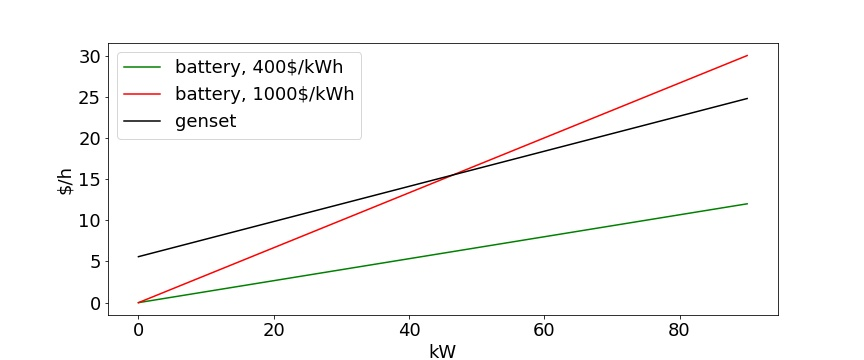
\includegraphics[scale=0.5]{energy_cost.jpeg}
\caption{Стоимость использования батареи и дизель-генератора}
\centering
\label{fig:bgcost}
\end{figure}

\medskip

Для нагрузки так же протестированы два значения: 70кВт и 30кВт.

Результаты представлены в Таблице \ref{t:res} и на Рисунках \ref{fig:res_70_400}, \ref{fig:res_70_1000} и \ref{fig:res_30} в Приложениях.
По результатам видно, что стратегии CC и СС2 незначительно отличаются при большой нагрузке и абсолютно эквивалентны при малой, поэтому для нагрузки 30кВт приведены только графики по CC. 
При дешёвой батарее лучшие результаты показывают CC и СС2, а при дорогой~--- LF, причем при малой нагрузке и дешёвой батарее разница существенна, а при остальных параметрах выражена менее явно.
Во всех случаях LF экономнее по отношению к ресурсу батареи, а СС~--- по отношению к топливу и моточасам.


\begin{table}[h]
\caption{Результаты применения стратегий на модели}
\label{t:res}
\begin{tabular}{{|p{1.9cm}|p{1.8cm}|p{2cm}|p{2cm}|p{2cm}|p{2cm}|p{2cm}|  }}
\hline
Стратегия & Нагрузка, кВт & Стоимость аккумулятора, \$/кВт ч & Остаток ресурса батареи, \% & Расход топлива, л & Количество часов работы дизель-генератора & Суммарные расходы, \$ \\
\hline
lf       & 70   & 400          & 99.89                & 1667             & 100       & 2022       \\
cc       & 70   & 400          & 99.18                & 1567             & 56        & 1974       \\
cc2      & 70   & 400          & 99.55                & 1645             & 72        & 1985       \\
lf       & 70   & 1000         & 99.9                 & 1660             & 97        & 2058       \\
cc       & 70   & 1000         & 99.69                & 1654             & 79        & 2154       \\
cc2      & 70   & 1000         & 99.82                & 1714             & 89        & 2136       \\
lf       & 30   & 400          & 99.9                 & 549              & 61        & 849        \\
cc       & 30   & 400          & 99.55                & 447              & 16        & 650        \\
cc2      & 30   & 400          & 99.55                & 447              & 16        & 650        \\
lf       & 30   & 1000         & 99.9                 & 542              & 58        & 882        \\
cc       & 30   & 1000         & 99.55                & 447              & 16        & 918        \\
cc2      & 30   & 1000         & 99.55                & 447              & 16        & 918      \\ 
\hline
\end{tabular}
\end{table}

\subsection{Задача выбора уставок мощности}
\label{sec:references}
    Двигаясь дальше, необходимо уточнить модель и постановку задачи для учёта изменчивого характера нагрузки и ветрогенерации. 
    Это окажет влияние на состав физической системы и обе подзадачи управления. 
    
    Поскольку мощность нагрузки и ветрогенерации может изменяться в реальном времени, задача выбора уставок должна решаться со значительно более высокой частотой, чем задача планирования.
    
    
    % Напомним, что мы разделили задачу управления на два этапа: 
    % \begin{enumerate}
    %     \item  Планирование.
    %     \item  Выбор уставок.
    % \end{enumerate}
    
    % \subsubsection{Планирование}
        % На этом этапе в соответствии с данным в разделе \label{sec:planning_problem} описанием задачи происходит планирование режима работы на следующий час.
        % Принципиальной ролью этого этапа является выбор оборудования, которое будет подготовлено к запуску и включено на весь следующий этап планирования, т.к. некоторые виды генераторов, систем аккумуляции и откладываемой нагрузки требуют время на подготовку к включению и выходу на рабочий режим и/или имеют ограничения на частоту включения/выключения, связанные с повышенным их износом при этих операциях.
        % Таким элементам соответствуют дискретные (бинарные) переменные оптимизационной задачи.
        % На данный момент сюда входит только дизельный генератор, в скором времени в модель также добавится система генерации и накопления водорода и протонно-обменный топливный элемент.
        
        % Второй (незадействованной на данный момент) функцией этого этапа является выдача постоянных референсных уставок оборудованию на весь период планирования, роль которых для получения глобально-оптимального управления будет обсуждена ниже.
        
        % Этап планирования реализован по стратегии LF, так же, как описано в предыдущем разделе, но с двумя отличиями: 
        % \begin{enumerate}
        %     \item  вместо реальной средней мощности ветрогенерации на следующий период используется \textit{наивное предсказание} равное среднему за предыдущий период,
            
        Чтобы учесть в этапе планирования колебания ветра и нагрузки в оптимизационную задачу \ref{f:lf} добавлено мягкое ограничение 
        maxGeneration - load~$\geq$ reserve 
        на обеспечение запаса мощности.
        Технически добавлена вспомогательная переменная $t$, одно ограничение типа неравенства и слагаемое в целевой функции:
        \begin{equation}
            \begin{split}
                x \cdot P_{genset~max} + P_{wind} - P_{battery~disch~max} + t &\geq P_{load} + P_{reserve}\\
                \Tilde{f} &= f + I \cdot t, ~ t \geq 0,
            \end{split}
        \end{equation}
    где $I$ --- достаточно большое число.
    
    
    Для компенсации кратковременных колебаний ветрогенерации в модель добавляется ещё один \textit{первичный} накопитель.
    Накопитель для долгосрочной аккумуляции энергии, состояние которого учитывается на этапе планирования, будем называть \textit{вторичным}.
    
    Выделять первичный накопитель в отдельное от вторичного накопителя устройство в принципе необязательно, например, если вторичный накопитель~--- литий-ионный аккумулятор.
    Однако это необходимо, если вторичный накопитель имеет недостаточно быстрый отклик на изменение уставки, как, например, водородные системы накопления (по результатам проведённых в НТЦ Автономной энергетики МФТИ испытаний коммерческого электролизного модуля, время переходных процессов до того, как электролизёр начинает отрабатывать уставку, составляет порядка одной минуты).
    Кроме того, может быть целесообразна установка суперконденсаторного накопителя в качестве первичного для снижения износа вторичного литий-ионного накопителя во время быстрых скачков мощности большой амплитуды \cite{mendis2013management, ju2017two}.
    
    В нашей модели инвертор первичного накопителя работает в астатическом по частоте и напряжению режиме и принимает на себя все колебания мощности.
    Все остальные управляемые устройства работают в режиме поддержания уставки.
    Это не самый элегантный механизм, но он наименее требовательный в плане разработки систем управления инверторами.
    
    Математически задача выбора уставок практически идентична задаче планирования по стратегии LF (задача \ref{f:lf}), за исключением двух отличий:
    \begin{enumerate}
        \item Бинарная переменная $x$  заменена на константу (выбранное на этапе планирование значение переменной $x$).  
        
        \item  Ограничение на баланс мощности модифицируется для учёта состояния первичного накопителя.
    \end{enumerate}
    
    Рассмотрим второй пункт подробнее.
    Необходимым условием сохранения физической устойчивости системы является поддержание уровня заряда первичного накопителя в той области, где он способен принимать на себя колебания мощности в системе.
    
    Поскольку первичный накопитель не принимает уставки мощности, управление его состоянием достигается за счёт выбора уставок остальным элементам системы. 
    
    Допустим, при проектировании системы было определено, что с целью экономии ресурса первичного накопителя, его SoE (SoE~--- State of Energy~--- отношение доступной для извлечения из батареи энергии к её номинальной энергетической ёмкости) должен находиться в диапазоне $[S_0, S_1]$.
    
    Этого можно добиться за счёт добавления к уставкам остальных устройств суммарной мощности равной мощности тока через первичный накопитель за последний период управления, когда SoE первичного накопителя выходит за допустимый диапазон и ``движется'' в направлении от центра допустимого диапазона.
    Точнее говоря, в описанных выше условиях к величине нагрузки на входе оптимизационной задачи добавляется следующее значение для корректировки заряда первичного накопителя:
    
    \begin{equation}
    \label{f:dL}
    \Delta L := E\cdot(SoE - SoE_{prev}) / \Delta t.
    \end{equation}
    
    В идеальных условиях (мгновенное и точное исполнение уставок оборудованием) это гарантирует, что отклонение энергии первичного накопителя от границы допустимого диапазона составит не более 
    
    \begin{equation}
    (\Delta P_{max} - \Delta P_{min})\Delta t, 
    \end{equation}
    где $\Delta P_{max}$, $\Delta P_{min}$  --- максимальная и минимальная возможные разности между мощностью нагрузки и мощностью ветрогенерации, $\Delta t$ --- период управления (период между обновлениями уставок).
    
    
    % Во-первых, штрафуется изменение каждой бинарной переменной(относительно её запланированного/текущего значения): 
    % на этапе коррекции в штатной ситуации не должно происходить включение оборудования, которому соответствуют дискретные переменные.
    % Переменные остаются переменными для случая резкого отклонения реальных погодных условий от прогнозированных. 
    % Вероятно, это должно быть заменено внеплановым вызовом алгоритма планирования.
    % Если бинарная переменная была равна 1 к началу очередной итерации коррекции, то она считается константой (в задаче нет жёстких ограничений, которые могли бы заставить платить штраф за смену значения дискретной переменной с 1 на 0).
    % В случае с одной дискретной переменной её значение может быть определено до решения оптимизационной задаче и в случае, когда она была равна 0 к началу итерации (из условия возможности соблюдения баланса мощности.
    
    
    % \textcolor{red}{П-регулятор для батареи не нужен. 
    % При кпд батареи = 1 при отсутствии регулятора энергия батареи будет колебаться в диапазоне шириной $P_{wind_max} \cdot \text{correctionTimeStep}$, повторяя профиль ветрогенерации (полностью поглощая колебания ветра). При кпд < 1 нужно лишь подзаряжать батарею примерно раз в день, когда кривая энергии батареи сползает вниз из-за потерь.
    % При этом остаётся проблема с тем, что при обеспечении нагрузки от батареи гибкости (дизель выключен, ветер в среднем меньше нагрузки) колебания ветра приводят к тому, что заряд перетекает между батареей гибкости и обратно.
    % Это неизбежно, если считать, что задача опорно-балансирующей батареи сделать так, как будто реальная ветрогенерация не отличается от той, что ожидалась при планировании(коррекции). 
    % Расчёт ожидаемой ветрогенерации по среднему за несколько последних периодов вместо одного улучшит ситуацию, в случае, когда в профиле ветра есть колебания значительной амплитуды с периодом равным периоду итерации коррекции (что наблюдается на наших данных, но общность под вопросом). Актуальные графики см в 1-year-hysteresis-dahsboard.ipynb в ветке milp}
    
    % Во-вторых, в целях поддержания заряда опорной батареи на уровне 50\%, значение нагрузки корректируется соответственно его отклонению.
    % Точнее говоря, к величине нагрузки (наивному предсказанию) на входе оптимизационной задачи добавляется выход пропорционального регулятора: 
    % \begin{equation}
    % \label{f:dL}
    % \Delta L := \alpha \frac{0.5 \cdot  \text{batteryMaxCharge} -
    % \text{batteryCharge}}{\text{correctionTimeStep}},
    % \end{equation}
    
    % где $\alpha$ --- настраиваемый коэффициент регулятора.
    % На тестовых данных его оптимальное значение (по критерию минимизации максимального отклонения заряда опорной батареи от 50\%) равно около $0.6$.
    
    Обратим внимание на смысл уставок, побочным образом получаемых в задаче планирования. 
    До сих пор мы их никак не использовали на этапе выбора уставок,  хотя кажется, что, будучи вычисленными для большего временного горизонта, чем на стадии выбора уставок, они могут давать полезную информацию для достижения долгосрочной оптимальности .
    
    Рассмотрим следующий пример.
    Допустим, получение мощности от батареи существенно дешевле получения мощности от дизель-генератора. Допустим также, что заряда батареи хватит чтобы покрыть ровно половину потребности в энергии на следующий период планирования.
    В таком случае для батареи и дизель-генератора на этапе планирования будут рассчитаны одинаковые уставки мощности, равные
    $L/2 = \text{batteryCharge} / \text{planningTimeStep}$.
    Допустим, что погода соответсвует прогнозу, и ветрогенерация на всем рассматриваемом периоде планирования достаточно близка к своему среднему.
    Тогда локально-оптимальный алгоритм выбор уставок в течении первой половины периода для батареи и генератора будет выбирать уставки $(L, 0)$, а вторую половину, когда батарея уже разрядится, $(0, L)$.
    Может показаться, что это плохо, но в случае линейных функций стоимости итоговые затраты за период не меняются. 
    Зато принуждение алгоритма выбора уставок к следованию референсным уставкам приводит к повышению затрат при существенном отклонении погоды от прогноза. 
    Поэтому на текущий момент уставки с этапа планирования не используются, но описанное в этом примере свойство поведения локально-оптимальных алгоритмов коррекции нужно иметь ввиду при переходе к нелинейным моделям.
    
    Для решения задачи не нужно иметь входные данные о нагрузке и ветрогенерации.
    Поскольку используется наивное предсказание, то нужны только данные о нагрузке и ветрогенерации, а точнее об их разности, за предыдущий период.
    Предполагая, что оборудование на предыдущем периоде строго следовало уставкам, получаем, что достаточно знать изменение  уровня заряда опорной батареи в начале данного и предыдущего периода планирования/коррекции 
    $\Delta E_{core~battery, i}$:
    
    \begin{equation}
    \label{f:dP}
    \Delta P := \Delta P_i =  
    P_{wind, i-1} - P_{load, i-1} 
    = -y_{i-1}  + (z_{+, i-1} + z_{-, i-1})
    + \frac{\Delta E_{core~battery, i}}{\Delta t} 
    \end{equation}
    
    C учётом \ref{f:dL} и \ref{f:dP} математическая формулировка задачи выбора уставок имеет вид (используются обозначения из \ref{par:lf}):
\begin{equation}%\label{}
\begin{split}
\vspace{-4mm}
&f =  -a_b z_- + b_g x + a_g y 
\rightarrow \min\limits_{(y, z_+, z_-) \in \R^3 }\\
\text{s.t. }&\\ 
    &\begin{cases}
    \Delta P - \Delta L + y = z_+ + z_-,~
    \sign(\Delta L) = \sign(SoE - S_{1/2}) \wedge SoE \notin [S_1, S_0] \\
    \text{ничего, иначе}
    \end{cases} \\
&y \leq x \cdot P_{genset~max},\\
&0 \leq y, \\
&0 \leq z_+ \leq P_{battery~ch~max}, \\
&-P_{battery~disch~max} \leq z_- \leq 0. \\
\end{split}
\end{equation} 

    Здесь $S_{1/2} = \frac{S_1 - S_0}{2}$.
    
    Если в результате резких изменений внешних условий допустимое множество задачи окажется несовместным, необходимо внеочередным образом перейти к этапу планирования, чтобы включить дизель-генераторы.

         
% \subsection{Результаты моделирования}
% \label{sec:references_numeric}
        
%     Для численного моделирования использовались интерполированные до одной минуты данные по ветрогенерации в Тикси.
    
%     Программная реализация на PuLP показала неудовлетворительное для проведения исследовательской работы время исполнения,
%     вероятно, по причине того, что решение оптимизационных задач внутри цикла на каждой итерации требовало от операционной системы создания нового процесса
%     (большинство практически применимых солверов в PuLP --- бинарники с интерфейсом командной строки).
%     Поэтому оптимизиционные задачи были переписаны в формате входных параметров для функции linprog модуля scipy.optimize.
%     На данный момент scipy не поддерживает дискретные переменные в задачах линейного программирования, поэтому на этапа планирования для выбора переменной включения дизель-генератора решались две оптимизационные задачи, в каждой из которых эта переменная считалась константой, а на этапе коррекции её значение определялось предварительно из условия соблюдения баланса мощности.
%     Это дало ускорение вычислений в $>7$ раз.
    
%     Результаты моделирования для батареи стоимостью 1000\$ / кВтЧ и 400\$ / кВтЧ показаны на рисунках \ref{fig:corr-1000} и \ref{fig:corr-400} соответственно.
%     Для LF-функции потерь $a'_b = k a_b$.
    
%     Как видно по результатам, в данных конфигурациях применение потенциального подхода не даёт выигрыша.
    
%     На рисунке \ref{fig:core} показан типичный график изменения заряда опорной батареи.
    
%     Ipynb с симуляцией и интерактивными графиками доступен по  \href{https://github.com/niquepolice/electro/blob/milp/milp.ipynb}{ссылке}.
    
    
%     \begin{figure}[h]
% 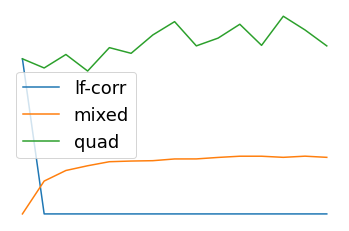
\includegraphics[scale=0.5]{/corr-1000d.png}
% \centering
% \caption{Зависимость итоговой стоимости от коэффициента k, 1000\$/кВт ч}
% \label{fig:corr-1000}
% \end{figure}

% \begin{figure}[h]
% 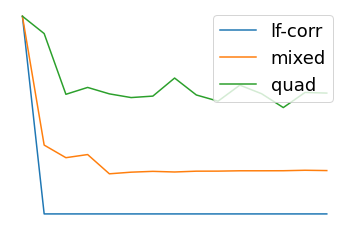
\includegraphics[scale=0.5]{/corr-400d.png}
% \centering
% \caption{Зависимость итоговой стоимости от коэффициента k, 400\$/кВт ч}
% \label{fig:corr-400}
% \end{figure}

% \begin{figure}[h]
% 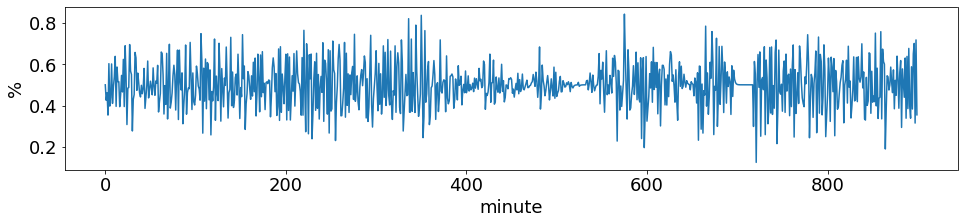
\includegraphics[scale=0.5]{/core.png}
% \centering
% \caption{График изменения заряда опорной батареи}
% \label{fig:core}
% \end{figure}


\subsection{Обзор продвинутых методов решения задачи планирования}

\begin{itemize}
    \item Учет нелинейностей \\
    Учёт нелинейности топливной характеристики дизель-генератора,
    зависимости износа батареи от глубины и тока заряда/разряда.
    В таком случае могут быть вычислительные проблемы с поиском точного решения методами выпуклой оптимизации.
    Применяются эвристические алгоритмы оптимизации, такие как алгоритм светлячка \cite{Sufyan2019}.
    
    \item Методы искусственного интеллекта\\
    Повышенный интерес к искусственному интеллекту и машинному обучению вкупе со сложностью поиска глобально-оптимальных решений в явном виде, приводит к существованию большого разнообразия подходов на основе методов искусственного интеллекта, например, генетических алгоритмов, нечёткой логики и полносвязных нейронных сетей \cite{Olatomiwa2016, kerdphol2016rbf, chaouachi2012multiobjective, jafari2018adaptive}.
    
    \item Model predictive control \\
    Хотя в литературе есть результаты, показывающие, что простые стратегии управления в некоторых случаях могут давать глобально-оптимальные решения \cite{Barley1996}, представляет интерес поиск универсальных глобально-оптимальных алгоритмов управления.
    Один из подходов, в которых явно заложен учёт оптимальности работы системы на следующих итерациях --- использование модельно-прогностического управления (Model Predictive Control, MPC).
    В статье \cite{Tazvinga2014} целевая функция MPC была составлена таким образом, чтобы минимизировать использование дизель-генератора и максимизировать использование ВИЭ; 
    было показано, что при наличии ошибок в прогнозировании потребления и генерации ВИЭ управление с помощью MPC на тестовой модели эффективнее управления с помощью квадратичного программирования (аналогично сформулированной выше задаче MILP для LF (\ref{f:lf}), только функция расхода дизеля имеет вид $aP^2 + bP$).
    
    \item Стохастическая оптимизация
    
    
    Пожалуй, в наиболее общем виде задача оптимального управления микрогридом может быть записана как задача минимизации матожидания затрат на эксплутацию системы на нескольких следующих периодах, то есть как задача стохастической оптимизации:
    \begin{equation}
        \E\left( \sum_{k=0}^m c_k ~\vert~ u_0 \right) \rightarrow \min\limits_{u_0},
    \end{equation}
    
    где $c_k$ --- затраты на $k$-ом интервале планирования, случайная величина, зависящая от вероятностных распределений случайных процессов ветрогенерации и нагрузки; $u_0$~--- управление на ближайший интервал.
    
    % Частными случаями такого подхода являются стратегии $CC$ и $LF$ --- при ветрогенерации равной нулю или достаточно большой константе соответственно.
    
    В статье Zeng P. et al. \cite{zeng2018dynamic} задача управления микрогридом в форме стохастической оптимизации решается методом приближенного динамического программирования (Approximate dynamic programming, ADP) с помощью рекуррентных нейронных сетей (Reccurent neural network, RNN).
    
    
    % \item Оперативная коррекция\\
    % Учёт возможности изменения нагрузки и ветрогенерации после планирования. 
    % Простейшее решение --- добавить в задачу оптимизации условие на наличие резерва мощности, доступного без включения на этапе оперативной коррекции новых генераторов.
    % При анализе решений задачи планирования для оценки эффективности по этому параметру (\textit{reliability analysis}) оценивают вероятность нехватки мощности \cite[8]{Sufyan2019} или вносят условие на её максимальное значение в ограничения оптимизационной задачи \cite[5]{Petersen2018}.
    
    \item Баланс реактивной мощности и задача об оптимальном потоке мощности\\
    При анализе физических процессов в системе мы ограничились уравнением баланса активной мощности, считая, что реактивная мощность в потреблении незначительна, и что физические соединения спроектированы таким образом, что мы можем не думать об ограничениях и потерях мощности в линиях.
    При необходимости, можно обратить внимание на баланс реактивной мощности \cite{zhang2016reactive} или рассмотреть более общую постановку задачи на основе уравнений потока мощности в сети \cite{kim2000comparison, molzahn2017survey}.
    
\end{itemize}

\newpage
\section{Специфика систем накопления энергии в разработке систем управления}


Как было описано в разделе \ref{sec:references}, в целевой физической системе все отклонения от предсказанных мощностей потребления и генерации компенсируются одним специально выделенным устройством --- первичным накопителем.
Назовём такую систему \textit{монобалансирующей}.
В монобаласирующей системе существует вероятность вероятность нежелательных перетоков энергии из первичного накопителя во вторичный и обратно, то есть циклы мощности внутри системы накопления энергии, как схематически изображено на Рис \ref{fig:power_flow_graph}.
Рассмотрим ситуацию, когда разность между мощностью нагрузки и мощностью ветрогенерации $P_{req}$  колеблется около нуля с периодом порядка периода выбора уставок.
Тогда, при неудачном выборе уставок мощности для вторичного накопителя (например, при прогнозе ветра равном среднему за предыдущий период) 
может получиться такой режим (см Рис \ref{fig:bad_batteries}),
что вторичный накопитель то заряжается от первичного в то время, как $P_{req} > 0$; то разряжается в первичный при $P_{req} < 0$ .


\begin{figure}[]
\begin{tikzpicture}[shorten >=1pt,node distance=2cm,on grid,auto]
  \tikzstyle{every state}=[fill={rgb:black,1;white,10}]

  \node[state, minimum size=2.2cm]  (w) at (0, 0)     {ветер};
  \node[state, minimum size=2.2cm]  (l) at (4, 0)     {нагрузка};
  \node[state, minimum size=2.2cm]  (s) at (2, -3)  {накопители};

  \path[->]
  (w) edge                node {}  (l)
  (w) edge                node {}  (s)
  (s) edge                node {$P_L$}  (l)
  (s) edge  [loop below]  node {$P_{ps}, P_{sp}$}  ();
\end{tikzpicture}
\centering
\caption{Диаграмма перетоков мощности}
\label{fig:power_flow_graph}
\end{figure}

\begin{figure}[]
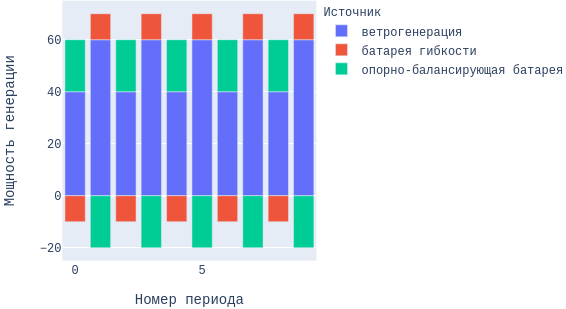
\includegraphics[scale=0.65]{/bad_batteries.png}
\centering
\caption{Плохой случай для системы с одним балансирующим устройством. Мощность нагрузки постоянна и равна 50кВт}
\label{fig:bad_batteries}
\end{figure}

Это приводит к лишнему износу накопителей и потерям энергии из-за $\eta < 1$.
Заметим, что в данном конкретном случае есть два принципиально различных ``хороших'' режима: 
\begin{enumerate}
    \item  Уставка вторичного накопителя $\equiv  0$.
    Все колебания сглаживаются первичным накопителем. 
    \item Вторичный накопитель идеально подстраивается под профиль ветра, первичный реагирует только на отклонения $P_{req}$ от своего среднего за период.
\end{enumerate}

У второго варианта два существенных недостатка: 
необходимость знать будущее и сохранение (неустранимой для монобалансирующей системы) проблемы с перетоками мощности в случае значительной дисперсии $P_{req}$ в периодах между обновлением уставок.
Недостаток первого варианта в том, что логически первичный накопитель предназначен только для компенсации колебаний внутри периода между выбором уставок.
В данном частном случае это исправляется увеличением этого периода вдвое.

Монобалансирующая система, использующая прогноз по предыдущему периоду, хороша тем, что с ней практически не нужно заботиться о поддержании заряда первичного накопителя в допустимом диапазоне:


% Поэтому достаточно, чтобы ширина рабочего диапазона опорно-балансирующей батареи $E_{core}(SoE_{max} - SoC_{min})$ была больше $\left(P_{req~max} - P_{req~min}\right)\Delta t$, тогда начало работы с состояния 
% $E_{core}(SoE(0) - SoC_{min}) = \left(P_{req}(i) - P_{req~max}\right)\Delta t $ гарантирует, что SoC будет находиться допустимом диапазоне при $\eta = 1$.
% При $\eta < 1$ нужно будет периодически подзаряжать опорно-балансирующую батарею для компенсации потерь.

Далее будем считать, что система работает без дизель-генератора, и что разность между ветрогенерацией и нагрузкой $P_{req}$ всегда можно удовлетворить за счёт вторичного накопителя, или  $P_{req}$ скорректирована таким образом, чтобы под них подходить (это нужно, чтобы не думать сейчас о случаях, когда, например, ветра слишком много и вторичный накопитель уже заряжен).  
Для простоты учёта баланса мощности будем также считать, что КПД накопителей равен 1 (хотя потери при перетоках между накопителями~--- как раз то, что заставляет нас рассматривать эту проблему).

Главный вопрос об эффективности монобалансирующих системах, который нас интересует: для каких $\alpha$ существует управление (уставка вторичному накопителю с отрицательным знаком, то есть положительная при разряде) $u(i) = f(P_{req}(0), \ldots, P_{req}(i-1))$, $E_{p}(SoE(i) - SoC(i-1)) = \left( u(i) - P_{req}(i)\right)\Delta t$ удовлетворяющее следующим условиям (*):
\begin{enumerate}
    \item $\forall i ~ SoE(i) \in [SoC_{min}, SoC_{max}] \eqdef [0, 1]$ (для удобства производим перемасштабирование, чтобы считать ширину допустимого диапазона равной ёмкости первичного накопителя) .
    \item Ограничение на максимально допустимую долю энергии, перешедшую из одной батареи в другую: $E_{ps} + E_{sp} < \alpha E_{L}  ~\forall \Vec{P}_{req}$, здесь $E_{ps}, E_{sp}$ --- энергия поступившая из первичного накопителя во вторичный и обратно, соответственно; 
  % мб $E_{L} + E_f$ ??
    $E_{L}$ ---  энергия, отданная нагрузке системой аккумуляторов.
    Это ограничение соответствует ограничению на потери энергии в ходе циклических перетоков мощности между накопителями.
\end{enumerate}

Здесь $p$ в индексах соответствует первичному накопителю (primary), $s$~--- вторичному (secondary).

% Рассмотрим режим работы, в котором дизель-генератор выключен и нагрузка обеспечивается батареей гибкости и ветрогенерацией.
% Идеализируем эту систему, предполагая, что начальная энергия батареи гибкости = 0, диапазон энергий = $(-\infty, \infty)$ (бесконечная ёмкость, бесконечный запас энергии в начальный момент).
Считая, как обычно, что мощность батареи положительна при заряде, в использованных выше обозначениях для данного случая получаем $u = -P_{s}$.
Тогда 

\begin{equation}
\label{f:Efc}
\frac{dE_{sp}}{dt} = 
\begin{cases}
u,& P_{req} \leq 0, u \geq 0,\\
ramp(u - P_{req}),& P_{req} \geq 0, u \geq 0,\\
0,& u \leq 0.
\end{cases}
\end{equation}

И, аналогично

\begin{equation}
\label{f:Ecf}
\frac{dE_{ps}}{dt} = 
\begin{cases}
-u,& P_{req} \geq 0, u \leq 0,\\
ramp(P_{req} - u),& P_{req} \leq0, u \leq 0,\\
0,& u \geq 0.
\end{cases}
\end{equation}

Здесь $ramp$~---функция, равная нулю, если агрумент отрицателен, и равная своему аргументу в противном случае. 
% Легко заметить, что при $P_{req}(i) = -u$

% 3 дня работы деградированного интеллекта студента 6 курса
Понятно, что при $P_{req} \equiv 0$, если были какие-то потоки энергии, то в условии 2 $\alpha = 1$. 
Но в таком случае при $u \equiv 0 $ будут нулевые перетоки энергии. 
Поэтому учитывать стоит только случаи, когда левая и правая части условия растут с течением времени.
Легко заметить, что справедливо следующее
\begin{Statement}
Пусть в начальный момент времени энергия опорной батареи находилась в середине допустимого интервала, система монобалансирующая с \textit{фиксированным} шагом времени.
Пусть $\forall i ~P_{req}(i) \in [P_{req~min}, P_{req~max}] \eqdef [-A, A]$. 
Тогда $\forall u$, удовлетворяющего (*), существует $P_{req}$ такое, что сумма $E_{ps} + E_{sp}$ неограниченно растёт с течением времени, и в условии 2 выполнено $\alpha > 0.5 = \alpha_0$.
\end{Statement}


\begin{proof}
Возьмём произвольное управление $u$, удовлетворяющее (*).
Построим для него такой профиль разности между нагрузкой и ветрогенерацией $P_{req}$, чтобы было выполнено \begin{equation}
\label{f:a_0}
    E_{ps} + E_{sp} \geq \alpha_0 E_{L}.
\end{equation}

Пусть $u(i) = f(P_{req}(0), \ldots, P_{req}(i-1))$. 
Положим $$
P_{req}(i) = \begin{cases}
A\cdot \sign(\frac{1}{2} - SoE_{p}), &|u_i| \leq \frac{A}{2}~ (i \in \I),\\
0, &|u_i| \geq \frac{A}{2}~ (i \in \K).
\end{cases}
$$
Обозначим $\Delta E(i)$ изменение энергии первичного накопителя на i-ом шаге.
Так как при $i \in \I$ $P_{req}$ старается увести SoE первичного накопителя за границы допустимого диапазона, то понятно, что
$$\sum_{i \in \K}{|\Delta E(i)|} \geq \sum_{i \in \I}{|\Delta E(i)|} -\frac{E_{p}}{2} ,$$
здесь $E_p$~--- ширина допустимого диапазона.
Это особенно очевидно, если воспользоваться симметрией допустимого диапазона относительно 0.5 (считать, что при переходе через 0.5 сверху вниз траектория энергии отражается), тогда на шагах из $\I$ SoE движется всегда вверх, а на шагах из $\K$ может двигаться в любом направлении.

Воспользовавшись этим и \ref{f:Efc}-\ref{f:Ecf}, получаем

$$
E_{fc} + E_{cf} %\geq \Delta t \sum_{i \in \K}{|u_i|} 
\geq \sum_{i \in \K}{|\Delta E(i)|} \geq 
\sum_{i \in \I}{|\Delta E(i)|} -  \frac{E_{p}}{2} \geq
\frac{1}{2} E_{L} - E_{p}.
$$
Первое неравенство следует из того, что на шаге с номерами $i \in \K$ нагрузка равна ветрогенерации, поэтому на изменение уровня энергии в первичном накопителе накопителе на этом шаге равно перетоку энергии между накопителями.
В последнем неравенстве используется, что обмен мощностью с системой накопления происходит только на шагах из $\I$, и энергия, переданная от системы накопления нагрузке составляет не менее половины энергии, просуммированной по всем обменам с системой накопления за вычетом, быть может, ширины допустимого интервала.


% Пусть прошло $k$ периодов.
% Обозначим $n \defeq |\mathcal{I}|,~ \mathcal{I} \defeq \{i : |u(i)| \leq A/2, i\leq k\}$, 
% $m \defeq |\mathcal{K}|,~ \mathcal{K} \defeq \{i : |u(i)| \geq A/2, i \leq k\}$.

% Докажем, что $n \leq 4m$.
% При $i \in \mathcal{I}$ энергия опорной батареи изменяется (по модулю) на величину $\Delta E \geq \frac{A}{2} \Delta t$ в сторону ближайшей границы допустимого интервала.
% При $i \in \mathcal{K}$ энергия меняется на величину $ \Delta E \leq 2A \Delta t$ в произвольную сторону.
% Отсюда очевидно, что при $n > 4m$ (с учётом начального условия) энергия батареи выходит за границы допустимого интервала, поэтому приходим к противоречию.

% Так как $E_{L} + E_f \leq \sum_i^k{|u(i)|}$ \textit{(мб можно улучшить оценку?)} и  при каждом $i \in \mathcal{K}$ выполнено $ E_{cf}(i) + E_{fc}(i) = |u(i)| \geq \frac{A}{2}$, то 
Из этого следует справедливость \ref{f:a_0} для $\alpha_0 = \frac{1}{2}$.
\end{proof}

Полученный результат говорит о том, что не существует системы управления монобалансирующей системой со многоуровневой системой накопления энергии, для которой перетоки мощности между накопителями были бы пренебрежимо малы при любых внешних условиях: в худшем случае не менее 50\% от энергии, поступающей в систему накопления испытывает двойные потери за счёт обмена энергией между накопителями.
Выводы из этого следующие:

\begin{enumerate}
    \item В качестве варианта по-умолчанию стоит рассматривать системы, где функции первичного и вторичного накопителя объединены в одном литий-ионном аккумуляторе.
    
    \item При создании систем с гибридной системой накопления энергии необходим анализ ожидаемых временных рядов разности ветрогенерации и нагрузки $P_{req}$, чтобы выбором параметров алгоритма управления по возможности минимизировать перетоки между накопителями (выбрать период между выбором уставок таким, чтобы циклы выбора уставок не накладывались на циклы $P_{req}$, убедиться в возможности минимизации перетоков). 
    
    \item При проектировании локальных системы управления устройствами силовой электроники следует закладывать возможность динамического изменения коэффициентов статизма, чтобы все накопители могли откликаться на колебания $P_{req}$ до вмешательства верхнеуровневой системы управления.
\end{enumerate}



\subsection{Износ батареи, подсчёт циклов}

 

Критерии оптимальности управления системой должны учитывать влияние управления на интенсивность износа оборудования.
До сих пор мы считали, что ресурс дизель-генератора равен матожиданию часов (моточасов) работы до необходимости замены/капитального ремонта и не зависит от характера эксплуатации при соблюдении технических требований, таких как ограничения на максимальную мощность и частоту включения выключения.
Относительно электрохимических накопителей мы предполагали, что их ресурс определяется количеством электрической энергии, которое может пройти через накопитель, до того, как его необходимо будет заменить (в этом предположении ресурс так же зависит только от одного параметра, не учитывающего многие особенности режима работы).

Если в оценке ресурса дизель-генераторов мы следуем общепринятой практике, то для электрохимических накопителей и литий-ионных батарей в частности наше предположение о модели деградации может быть недостаточно обосновано.

Действительно, в большинстве приложений (мобильные устройства, транспорт, источники бесперебойного питания) аккумуляторы используются глубокими циклами заряда-разряда, поэтому производители измеряют ресурс аккумулятора в количестве циклов до замены. 
Поскольку опорный накопитель в монобалансирующей системе часто испытывает изменение величины и направления протекающего через него тока, возникает вопрос о влиянии циклов малой глубины (\textit{микроциклов}) на износ батареи.

В отсутствии общепризнанных моделей деградации, учитывающих величину тока (C-rate), глубину цикла (Depth of discharge, DoD) и его положение (SoC mean) \cite{laresgoiti2015modeling}, определить влияние микроциклов на ресурс батареи можно только путём проведения натурных испытаний или физико-химического моделирования. 
Для этого необходимо численно описать типичный режим работы опорного накопителя в терминах количества и глубины циклов.

Далее будет описано два способа построения ненормированной эмпирической функции распределения глубины циклов $nF(d)$~--- практически очевидный метод подсчёта количества циклов глубины более $d$ и алгоритм \textit{rainflow}, известный в русской литературе как \textit{метод дождя}, причем последний по-видимому впервые описывается на русском языке в удобном для программной реализации виде (с псевдокодом и реализацией на Python3).
Далее приведены результаты применения этих алгоритмов на данных, полученных моделированием работы энергосистемы.

\begin{enumerate}
\item Точечная оценка $nF(d)$

Наиболее простой и грубый способ, как с алгоритмической точки зрения, так и в плане точности получаемых результатов.
Входными данные для обоих алгоритмов --- зависмость SoC или SoE от времени, обозначим её $s(t_i)$.
Для удобства будем считать, что измерения проводятся с одинаковым интервалом $\Delta t$, тогда без потери информации можем параметризовать входные данные номером измерения: $s(i)$.
Назовём циклом глубины $d$ последовательность идущих подряд измерений $\{s(i)\}_{i=k}^{r}$, такую, что 
$\exists m,~ k \leq m \leq r$ 
и либо $s(m) - s(k) \geq d ~\wedge~ s(m) - s(r) \geq d$ (цикл заряда-разряда), либо
 $s(k) - s(m) \geq d ~\wedge~ s(r) - s(m) \geq d$ (цикл разряда-заряда).
 
Отсюда очевиден способ подсчитать количество циклов глубины более $d$, то есть получить значение величины $n(1 - F(d))$: в процессе прохода по массиву, обновляя индексы, соответствующие локальному максимуму ($h$) и локальному минимуму ($l$), проверять, не образует ли текущее измерение вместе с измерениями $h$ и $l$ цикл глубины $ > d$.
Соответствующий псевдокод:

\begin{algorithm}
\caption{Точечная оценка $n(1 - F(d))$}\label{alg:simple-cycle}
\hspace*{\algorithmicindent} \textbf{Input:} s(i)~--- анализируемый массив, n~--- количество элементов в массиве, d~--- минимальная глубина цикла \\
\hspace*{\algorithmicindent} \textbf{Output:} cycles~--- количество циклов глубины более d 

\begin{algorithmic}[1]
\State $cycles, i, l, h \gets 0$

\While{$i < n$}

\If {$s(h) - s(l) > d \And (l > h \And s(i) - s(l) > d \Or 
l < h \And s(h) - s(i) > d)   $}
    \State $l,h \gets i$
    \State $cycles \gets cycles +1$
\Else
    \If {$s(i) > s(h)$}
        \State $h \gets i$
    \EndIf
    \If {$s(i) < s(l)$}
        \State $l \gets i$
    \EndIf
\EndIf
\State $i \gets i+1$
\EndWhile
 
\end{algorithmic}
\end{algorithm}

Очевиден недостаток этого способа~--- число проходов по массиву равно желаемому числу точек на графике $nF(d)$.
Другая проблема в том, что алгоритм обходит стороной сложности, возникающие при попытке разбиения массива $s(i)$ на циклы.
Как минимум, логика алгоритма допускает, что часть измерений может не принадлежать никакому циклу: действительно, алгоритм считает, что цикл ограничен точками $l, i$ или $h, i$, а переменные $l$ и $h$ могут обновляться в процессе поиска следующего цикла, оставляя между собой и правой границей последнего цикла никуда не определённые измерения.

\item Разбиение массива на циклы, алгоритм rainflow.

При разбиении массива на циклы возникает вопрос, как определить ``правильное'' разбиение.
На графике $s(i)$ внутри циклов большей глубины могут находиться вложенные циклы меньшей глубины, и количество уровней вложения может быть произвольным.
Разбиение всегда можно провести разными способами, причем мультимножества глубин циклов, полученные этими способами, не обязательно должны совпадать.

Рассмотрим случай, изображенный на Рисунке \ref{fig:nested-cycle}.
Здесь мы видим глубокий внешний цикл разряда-заряда, и вложенный цикл, который допускает как минимум два естественных представления: как цикла заряда-разряда $b-c-f$ и как цикл разряда-заряда $c-d-g$.
В первом случае внешний цикл $a-bf-d-e$ разрывается в точках $b$ и $f$, соответствующих одному и тому же значению $s(i)$, во втором случае внешний цикл образуется последовательностью точек $a-b-cg-e$.
Стоит заметить, что мы получили два разбиения на циклы разной глубины: во втором случае внешний цикл имеет минимум в точке $b$, поэтому его глубина меньше, чем у внешнего цикла в первом разбиении.


\begin{figure}[h]
\centering
\begin{subfigure}[b]{0.45\textwidth}
\centering
\begin{tikzpicture}
% \draw (0,0) -- (1,-3) -- (2, -2) -- (3, -4) -- (5, 0) ;
\filldraw [line width=0.25mm]
(-0.5, -0.5) --
(0,0) circle (2pt) node[left] {a} --
(1,-3) circle (2pt) node[align=center,   below] {b} -- 
(2, -2) circle (2pt) node[above] {c} -- 
(3, -4)  circle (2pt) node[below] {d} -- 
(5, 0) circle (2pt) node[right] {e} --
(5.5, -0.7);

\filldraw [line width=0.15mm, dashed]
(2, -2) -- 
(4, -2)  circle (2pt) node[right] {g};

\filldraw [line width=0.15mm, dashed]
(1, -3) -- 
(2.5, -3)  circle (2pt) node[right] {f};
\end{tikzpicture}
\caption{Способы разбиения на вложенный цикл и внешний}
\label{fig:nested-cycle}
\end{subfigure}
\hfill
\begin{subfigure}[b]{0.45\textwidth}
\centering
\begin{tikzpicture}
% \draw (0,0) -- (1,-3) -- (2, -2) -- (3, -4) -- (5, 0) ;
\filldraw [line width=0.25mm]
(0,0) circle (2pt) node[left] {a} --
(2,-4) circle (2pt) node[align=center,   below] {b} -- 
(4, 0) circle (2pt) node[right] {c};

\filldraw [line width=0.15mm, dashed]
(1, -2) circle (2pt) node[left] {d} -- 
(3, -2)  circle (2pt) node[right] {e};
\end{tikzpicture}
\caption{Разбиение цикла на два подцикла}
\label{fig:one-cycle}
\end{subfigure}
\caption{Примеры неоднозначности разбиения на циклы}
\end{figure}

Вообще говоря, без надлежащих оговорок, даже график с единственным циклом можно разбить на несколько циклов: на Рисунке \ref{fig:one-cycle} цикл $a-b-c$ разбивается на два цикла $a-de-c$ и $d-b-e$.
Очевидно, что подобным образом можно получить бесконечное количество разбиений одного цикла на любое число циклов.

В обоих рассмотренных выше примерах дополнительные варианты разбиения имели меньшую глубину внешнего цикла, чем некоторый экстремальный вариант.
Предполагая, что циклы меньшей глубины в меньшей степени расходуют ресурс накопителя, мы хотели бы получить разбиение, которое сохраняет максимально глубокие циклы.
Исторически алгоритмы rainflow, к одному из вариантов которого мы сейчас приближаемся, разрабатывались для анализа усталостных нагрузок металлов при циклических деформациях, при которых влияние на ресурс также зависит от глубины деформации.
Но в настоящее время использвуется и для анализа деградации аккумуляторных батарей в научной литературе \cite{xu2016modeling}.

Пожалуй, проще описать алгоритм, и ввести определение ``правильного'' разбиения на циклы на основе свойств этого алгоритма, чем давать их явное математическое описание.
Так, например, в статье \cite{rychlik1987new} приводится новый алгоритм подсчёта циклов, более явная форма описания которого удобна для теоретического анализа распределений циклов, формируемых случайным процессом внешнего воздействия.
Корректность нового алгоритма обосновывается доказательством того, что он даёт тот же результат, что и алгоритм rainflow, впервые предложенный в статье \cite{matsuishi1968fatigue} без четкого математического описания постановки задачи.
Попытка простого описания алгоритма rainflow в разных формах также предпринята в работе \cite{downing1982simple}.

Сейчас мы опишем алгоритм rainflow, принимающий на вход массив $s(i)$ измерений SoC или SoE и возвращающий массив $d(i)$ глубин циклов.
При желании учитывать в модели деградации средний модуль тока за цикл, предложенный алгоритм несложно модифицировать, добавив во входные данные массив времени регистрации измерений $t(i)$, а в выходные данные~--- массив длительностей циклов $\tau(i)$.

На русском языке ``Метод дождя'' принципиально описан в Стандарте 
``МЕТОДЫ СХЕМАТИЗАЦИИ СЛУЧАЙНЫХ ПРОЦЕССОВ НАГРУЖЕНИЯ ЭЛЕМЕНТОВ МАШИН И КОНСТРУКЦИЙ И СТАТИСТИЧЕСКОГО ПРЕДСТАВЛЕНИЯ РЕЗУЛЬТАТОВ'' 
ГОСТ 25.101-83, однако перевести данное в нём описание в код~--- не самая очевидная процедура.
Здесь же мы приведём псевдокод алгоритма, а с реализацией на Python3 можно ознакомиться в репозитории-приложении к работe \hyperlink{https://github.com/niquepolice/master-thesis-code/blob/master/cycles.ipynb}{по ссылке}.

Принцип работы алгоритма следующий. 
Сначала выполняется подготовительная процедура, удаляющая горизонтальные участки из графика $s(i)$ (это нужно для того, чтобы можно было определять, является ли точка локальным экстремумом, глядя лишь на значения $s(i)$ в двух соседних точках).

Далее инициализируются два изначально пустых стека (LIFO-структура данных) $min$ и $max$ для хранения индексов локальных экстремумов.
В процессе прохода по массиву каждая точка проверяется на локальный экстремум.
Если найден локальный максимум, производится ``схлапывание'' циклов разряда-заряда: если последний найденный максимум (лежащий на вершине стека $max$) не выше текущего, то он ``схлапывается вправо''~--- из стеков $min$ и $max$ удаляется по одной точке, фиксируется цикл глубины, равной модулю разности значений $s(i)$ в удалённых точках.
Это повторяется, пока на вершине стека $max$ не окажется максимум, лежащий выше текущего. 
После этого в стек $max$ добавляется текущий максимум.
Таким образом, в стеке $max$ всегда находится возрастающая последовательность локальных масимумов (если смотреть с вершины стека).
Симметричная ситуация происходит с локальными минимумами. 


\begin{figure}[]
\centering
\begin{subfigure}[b]{0.45\textwidth}
    \centering
    \begin{tikzpicture}
    % \draw (0,0) -- (1,-3) -- (2, -2) -- (3, -4) -- (5, 0) ;
    \filldraw [line width=0.25mm]
    (-0.5, -0.5) --
    (0,0) circle (2pt) node[left] {a} --
    (1,-3) circle (2pt) node[align=center,   below] {b} -- 
    (2, -2) circle (2pt) node[above] {c} -- 
    (3, -4)  circle (2pt) node[below] {d} -- 
    (5, 0) circle (2pt) node[right] {e} --
    (5.5, -0.7);
    
  \draw[-{Latex[length=3mm, width=2mm]}, dashed]
  (2,-2) -- (2/3, -2);
    \end{tikzpicture}
    % \caption{Способы разбиения на вложенный цикл и внешний}
\end{subfigure}
\begin{subfigure}[b]{0.45\textwidth}
    \centering
    \begin{tikzpicture}
    % \draw (0,0) -- (1,-3) -- (2, -2) -- (3, -4) -- (5, 0) ;
    \filldraw [line width=0.25mm]
    (-0.5, -0.5) --
    (0,0) circle (2pt) node[left] {a} --
    (1.5, -2) circle (2pt) node[above] {c} -- 
    (2.25,-3) circle (2pt) node[align=center,   below] {b} -- 
    (3, -4)  circle (2pt) node[below] {d} -- 
    (5, 0) circle (2pt) node[right] {e} --
    (5.5, -0.7);
    
  \draw[-{Latex[length=3mm, width=2mm]}, dashed]
  (5,0) -- (0, 0);
    \end{tikzpicture}
    % \caption{Способы разбиения на вложенный цикл и внешний}
\end{subfigure}

\caption{``Схлапывание'' в алгоритме rainflow.}
\label{fig:cycles-сollapse}
\end{figure}

Для примера рассмотрим ситуацию на Рисунке~\ref{fig:cycles-сollapse}.
При достижении минимума в точке b и максимума в точке $c$ ``схлапываний'' не происходит,
%~--- предыдущий максимум в точке $a$ выше текущего, в 
локальные экстремумы просто помещаются в  соответствующие стеки.
При достижении минимума в точке $d$, лежащего ниже точки $b$, 
индексы,  соответствующие точкам $b$ и $c$ удаляются из стеков,
вложенный цикл $c'-b-c$ как бы ``схлапывается влево'', 
оставляя один внешний цикл $a-d-e$, который затем ``схлопнется'' при достижении точки $e$. 

Если повернуть Рисунок \ref{fig:cycles-сollapse} на $\pi/2$, то картина схлапывающихся циклов может напомнить стекание воды по крышам пагоды (Рисунок \ref{fig:pagoda}).
Алгоритм rainflow, описанный через стекание воды по крышам пагоды, называется \textit{Pagoda roof method}.
Именно таким образом алгоритм вводится в ГОСТ 25.101-83.

\begin{figure}
    \centering
    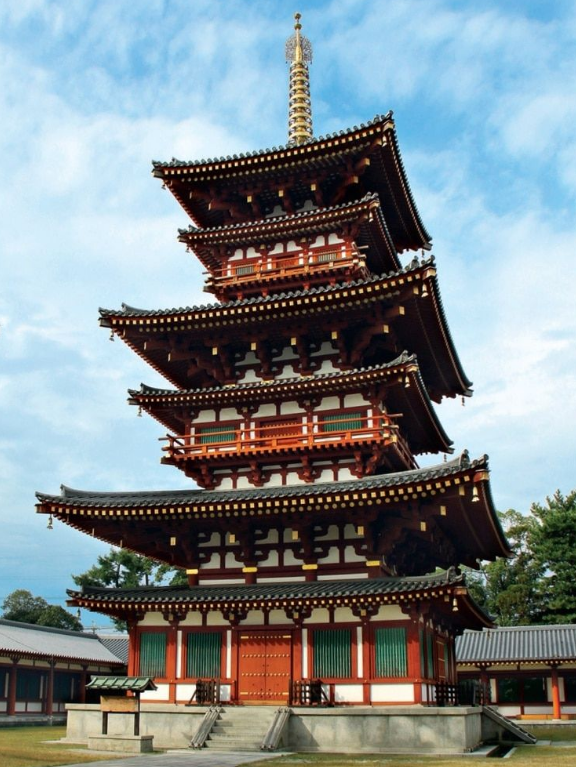
\includegraphics[scale=0.3]{pics/pagoda.png}
    \caption{Фотография пагоды. Изображение взято с сайта https://www.pinterest.cl/pin/405394403957944422/}
    \label{fig:pagoda}
\end{figure}

\begin{algorithm}
\caption{Алгоритм Rainflow}\label{alg:rainflow}
\hspace*{\algorithmicindent} \textbf{Input:} s(i)~--- анализируемый массив, n~--- количество элементов в массиве \\
\hspace*{\algorithmicindent} \textbf{Output:} d(i)~--- массив глубин циклов 
\begin{algorithmic}[1]
% \State $cycles, i, l, h \gets 0$

\State $i,k \gets 1$
\While{$i < n$} \Comment{удаляем горизонтальные участки}
\If {$s(i) \neq s(i-1)$}
    \State $s(k) \gets s(i)$ 
    \State $k \gets k + 1$
\EndIf
\State $i \gets i + 1$
\EndWhile
\State{$n = k$}
\Statex

\Function{collapse\_last}{$max, min, s$} \Comment{``Схлапывает'' последний цикл, возвращает его глубину}
\State{$depth \gets s(max$.pop())$ - s(min$.pop())}
\State{\textbf{return} $depth$ }
\EndFunction
\Statex

\State{$i \gets 1$}
\State{$d \gets$ пустой список/массив}
\State{$min, max \gets$ пустые стеки}
\While{$i < n-1$}
\If{$s(i) > s(i-1) \And s(i) > s(i+1)$}
    \While{$max$ не пуст $\And s(i) >= s(max$.top()) } \Comment{Сравниваем текущее значение со значением предыдущего максимума}
        \State{$d$.append(COLLAPSE\_LAST($max, min, s$))} 
    \EndWhile
    \State{$max$.append($i$)}
\EndIf
\If{$s(i) < s(i-1) \And s(i) < s(i+1)$}
    \While{$min$ не пуст $\And s(i) <= s(min$.top()) } 
        \State{$d$.append(COLLAPSE\_LAST($max, min, s$))}
    \EndWhile
    \State{$min$.append($i$)}
    
\EndIf
\State{$i \gets i + 1$}
\EndWhile
 
\end{algorithmic}
\end{algorithm}

\end{enumerate}

Теперь приведём сравнение результатов применения обоих методов подсчёта циклов.

Для анализа использовался массив SoE опорной батареи (см Рисунок \ref{fig:core-cycles-line}), полученный путем моделирования на RTDS работы энергосистемы, состоящей из ветрогенератора, постоянной нагрузки, опорной батареи и нескольких других накопителей (модель разрабатывалась в рамках проектов Инжинирингового центра автономной энергетики МФТИ).
Моделирование длилось около 6 часов, для анализа использовались записи измерений с периодом 1 секунда.

\begin{figure}[h]
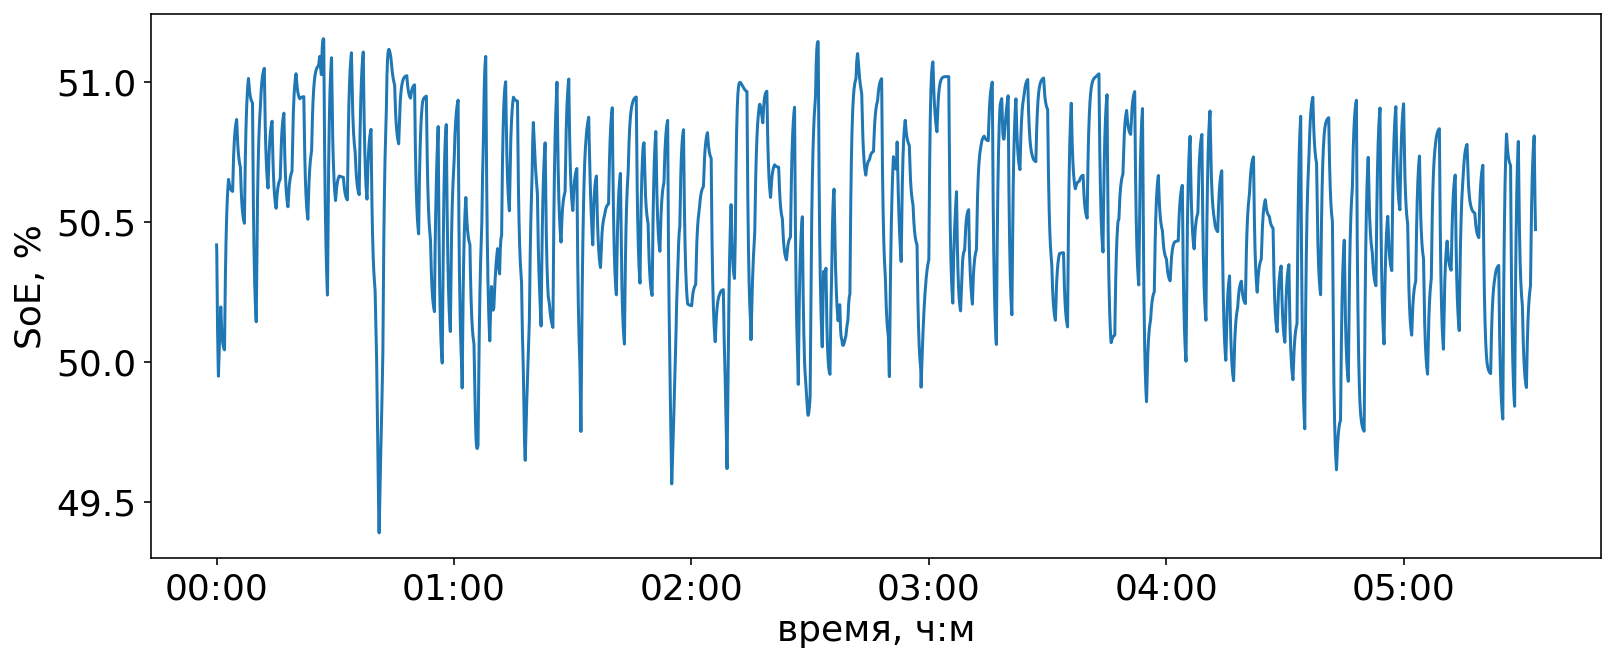
\includegraphics[scale=0.55]{/cycles_soe.png}
\caption{График SoE опорной батареи, использовавшийся в качестве входных данных для тестирования алгоритмов подсчёта циклов}
\centering
\label{fig:core-cycles-line}
\end{figure}

\medskip

Гистограмма глубин циклов, полученная алгоритмом Rainflow, представлена на Риснуке \ref{fig:cycles-hyst}.
По ней можно получить представление о характере работы опорной батареи в системе.
Видно, что распределение циклов практически однородное от циклов нулевой глубины до циклов максимальной глубины в ~1.5\% за исключением пика распределения около нуля, который может быть связан с шумом в измерениях.

\begin{figure}[h]
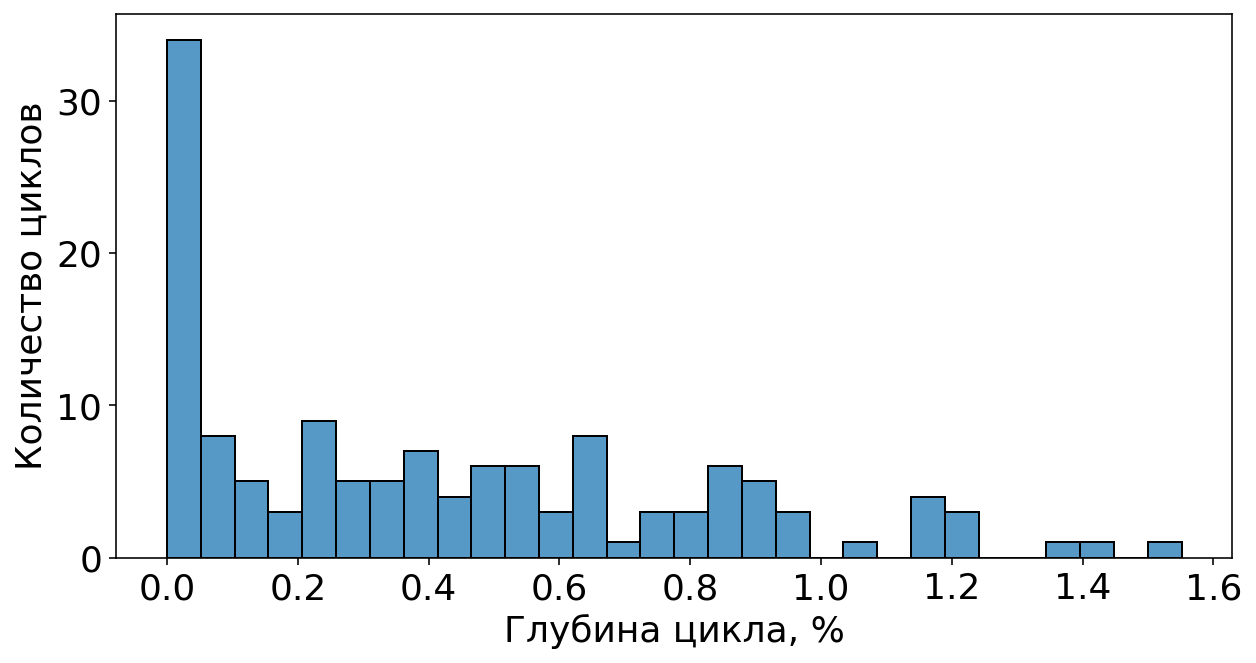
\includegraphics[scale=0.7]{/cycles_hyst.png}
\caption{Гистограмма глубин циклов, полученная алгоритмом Rainflow}
\centering
\label{fig:cycles-hyst}
\end{figure}


\begin{figure}[h]
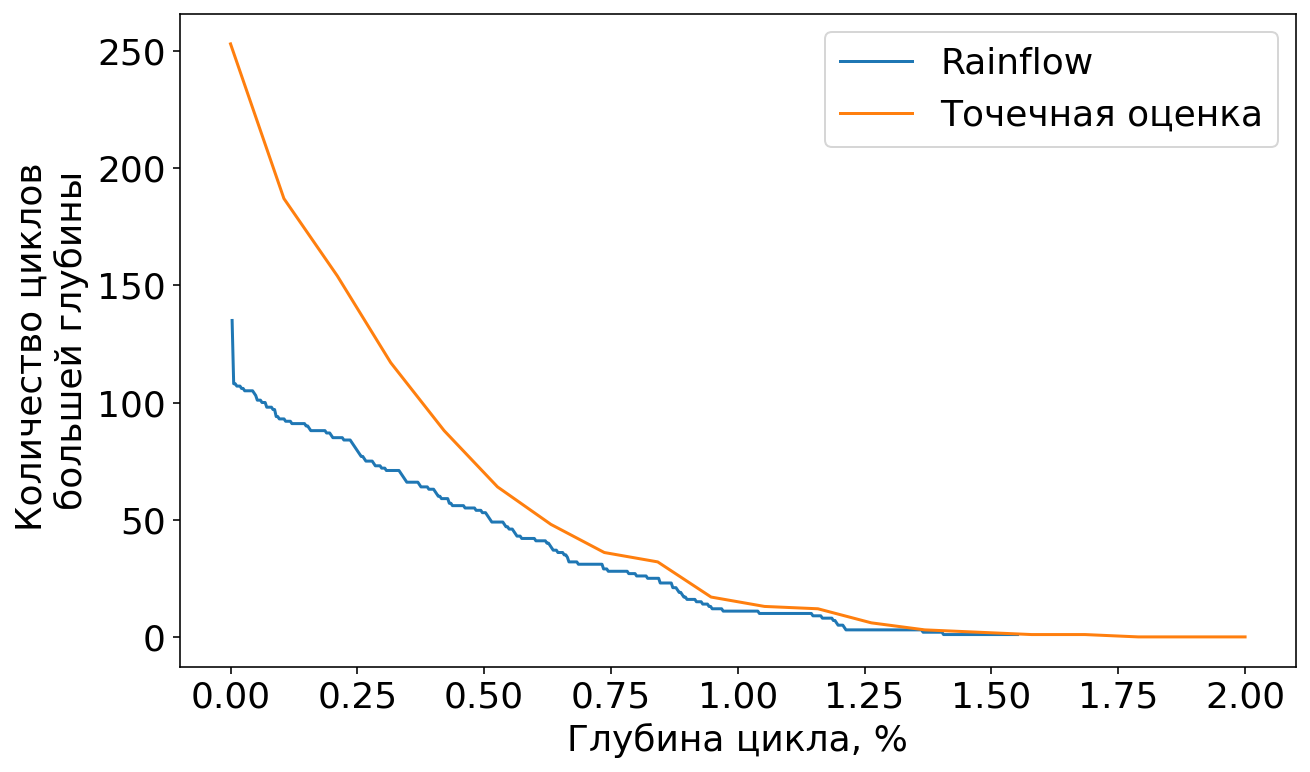
\includegraphics[scale=0.55]{/cycles_two_methods.png}
\caption{Результаты подсчёта количества циклов глубины более $d$ двумя методами}
\centering
\label{fig:cycles-two-methods}
\end{figure}


\begin{figure}[h]
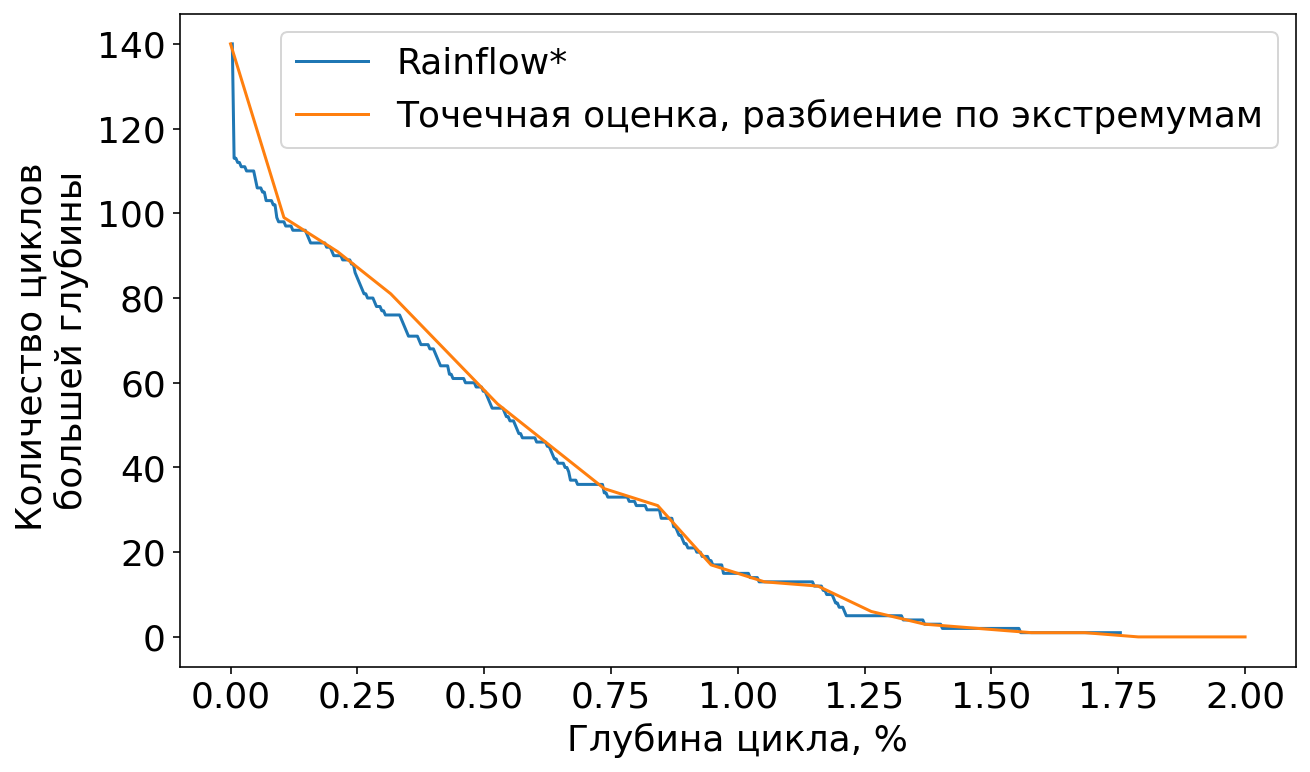
\includegraphics[scale=0.55]{/cycles_two_methods_2.png}
\caption{Результаты подсчёта количества циклов глубины более $d$ методом точечной оценки с разбиением по экстремумам и алгоритмом Rainflow с подсчетом остаточных циклов}
\centering
\label{fig:cycles-two-methods-2}
\end{figure}

Результаты подсчёта количества циклов глубины более $d$ (величины $n(1 - F(d))$) представлены на Рисунке \ref{fig:cycles-two-methods}.
Видно, что для циклов большой глубины результаты упрощённого метода, хотя и менее детализированы, но примерно совпадают c результатами Rainflow.
Но количество подсчитанных циклов малой глубины различается практически в два раза.
Это связано с тем, что простой Алгоритм \ref{alg:simple-cycle} разбивает циклы на два цикла меньшей глубины.
Например, если $s(t)$~--- треугольная повторяющаяся волна, Алгоритм \ref{alg:simple-cycle} для $d=0$ подсчитает по одному циклу вокруг каждого экстремума (получатся чередующиеся циклы заряда-разряда и разряда-заряда в два раза меньшей глубины, чем амплитуда колебаний), и подсчитанное количество циклов будет в два раза больше числа длин волн в $s(t)$.
Чтобы исправить этот недостаток, можно проверять условие завершения цикла только в локальных экстремумах.
Ниже приведён Алгоритм \ref{alg:simple-cycle-extremums}~--- модифицированный с учетом этого замечания вариант Алгоритма \ref{alg:simple-cycle}.




\begin{algorithm}
\caption{Точечная оценка $n(1 - F(d))$, разбиение по экстремумам} \label{alg:simple-cycle-extremums}
\hspace*{\algorithmicindent} \textbf{Input:} s(i)~--- анализируемый массив без подряд идущих повторяющихся значений (горизонтальных участков на графике), n~--- количество элементов в массиве, d~--- минимальная глубина цикла \\
\hspace*{\algorithmicindent} \textbf{Output:} cycles~--- количество циклов глубины более d.

\begin{algorithmic}[1]
\State $cycles, l, h \gets 0$
\State $i \gets 1$

\While{$i < n - 1$}

\If{$s(i) > s(i-1) \And s(i) > s(i+1)\Or s(i) < s(i-1) \And s(i) < s(i+1)$}
    \If {$s(h) - s(l) > d \And (l > h \And s(i) - s(l) > d \Or 
    l < h \And s(h) - s(i) > d)   $}
        \State $l,h \gets i$
        \State $cycles \gets cycles +1$
    \Else
        \If {$s(i) > s(h)$}
            \State $h \gets i$
        \EndIf
        \If {$s(i) < s(l)$}
            \State $l \gets i$
        \EndIf
    \EndIf
\EndIf
\State $i \gets i+1$
\EndWhile
 
\end{algorithmic}
\end{algorithm}

Небольшое превышение количества подсчитанных Алгоритмом \ref{alg:simple-cycle} глубоких циклов по сравнению с Алгоритмом \ref{alg:rainflow} (Rainflow) связано с тем, что после окончания работы Алгоритма \ref{alg:rainflow} в стеках $min$ и $max$ остаются вершины, ещё не ``схлопнутые'' в какой-либо цикл. 
Обычно этот ``остаток'' не накапливается при увеличении длины массива $s(i)$, поэтому для достаточно больших массивов им можно пренебречь, что и сделано в Алгоритме \ref{alg:rainflow}, чтобы не заниматься интерпретациями этих ``остатков''.
Однако для более справедливого сравнения двух методов, добавим в конец  Алгоритма \ref{alg:rainflow} подсчет оставшихся неучтенными циклов:
\begin{algorithmic}
\While{$min$ не пуст $\And max$ не пуст} 
\State{$d$.append(COLLAPSE\_LAST($max, min, s$))}
\EndWhile
\end{algorithmic}

Результаты сравнения Алгоритма \ref{alg:simple-cycle-extremums} и алгоритма Rainflow с подсчетом остаточных циклов представлены на Рисунке \ref{fig:cycles-two-methods-2}.
Теперь полученные обоими методами кумулятивные распределения глубин циклов практически совпадают.
Заметно, что расчеты Rainflow значительно детализированнее, кроме того он вычислительно эффективнее: однопоточная имплементация на Python3 требует для вычисления методом Rainflow в среднем около 0.15 секунд Intel® Core™ i7-8700, а расчёт 20 точек методом точеченой оценки~---1.7 cекунды.

% \section{Распределённые системы управления}
\label{sec:distributed}

https://ieeexplore.ieee.org/abstract/document/8585956 --про суперконденсаторы.
 Секция 3 --- обзор алгоритмов частотного разделения лития и суперкапов, мультиагентные системы

\url{https://ieeexplore.ieee.org/stamp/stamp.jsp?tp=&arnumber=4497237&tag=1}
Distributed MPC Strategies With Application to Power System Automatic Generation ControlAswin N. Venkat,  Ian A. Hiskens, 
--- Communication-Based MPC $\rightarrow$ равновесие Нэша.\\
Feasible Cooperation-Based MPC

\url{https://www.youtube.com/watch?v=e_DlQhe3yiI}
--- распределённая стохастическая оптимизация на сетях.
Выбор случайных соседей (входная степень не больше Q) чтобы уменьшить количество рёбер в подграфе передачи данных 17минута (исходный граф может быть полным), gossip как аналог случаю при Q=1

\url{https://ieeexplore.ieee.org/stamp/stamp.jsp?tp=&arnumber=9198090} Simultaneous Perturbation Stochastic Approximation-based Consensus for Tracking under Unknown–but–Bounded Disturbances Oleg Granichin,Senior Member, IEEE,Victoria Erofeeva, Yury Ivanskiy,and Yuming Jiang,Senior Member, IEEE --- ссылки в интро на историческую литературу про распределённую оптимизацию, consensus, gossip, что-то про невыпуклый случай

Мотивация к применению распределённых систем управления следующая:

\begin{itemize}
% \item
% Низкая инерция современных энергосистем требует высокой скорости реакции системы управления.
% Хотя это требование больше относится к первичному и вторичному регулированию

\item
При большом количестве устройств централизованное управление приводит к большим потокам данных через управляющий узел, что приводит к высоким (и растущим по мере подключения новых устройств) требованиям к сетевой инфраструктуре.
В модели распределённого управления агенты обмениваются информацией только с соседями по графу коммуникаций.
Отсутствие выделенного центрального узла позволяет избежать возникновения узкого места по мере расширения сети.
По литературе (\cite{binetti2014distributed} $\rightarrow$ \cite{elsayed2014fully}) также кочует мнение, что децентрализованные системы гибче по отношению к изменениям в сетевой топологии, поэтому лучше приспособлены к поддержке технологии plug-and-play.

\item
В распределённых системах управления сложность решения оптимизационной задачи делится между агентами, что может увеличить скорость вычислений для больших систем.

\item
Распределённое управление существенно надёжнее, так как не подвержено риску коллапса управляемой системы при отказе одного вычислительного узла.

\item
Распределённый подход позволяет не предоставлять центральному узлу информацию о своих измерениях, функциях стоимости и ограничениях, что обеспечивает приватность данных.
Также считается \cite{loia2013decentralized,molzahn2017survey} что распределённые системы надёжнее в плане кибербезопасности.

\item
Централизованный подход требует качественной модели системы (которая для большой системы становится слишком сложной), ошибки в модели приводят к плохому управлению \cite{binetti2014distributed}.


\end{itemize}
% В обзоре \cite{olivares2014trends} дана хорошая картинка разнообразия систем управления и их классификация, как по уровню в иерархии, так и по степени централизованности. 


Ниже дан обзор современных исследований в группе распределённых систем управления на уровне решения задач economic dispatch / optimal power flow. 
Эти два термина соответствуют двум близким постановкам задач. 
Первый обычно применяется для более идеализированной модели баланса активной мощности без потерь в линиях, второй --- когда учитываются импедансы линий и, соответственно, разница между амплитудами и/или фазами напряжений на шинах. 
\begin{itemize}
\item Распределённые алгоритмы численной оптимизации:
\begin{itemize}
% \item \cite{elsayed2014fully} --- распределённая оптимизация с невыпуклыми функциями стоимости. Цитирует
\item \cite{loia2013decentralized} --- в статье дано подробное иллюстративное описание централизованного подхода на методе Лагранжа. 
Предложен децентрализованный абсолютно симметричный подход к поиску решения задачи минимизации.
В основе метода лежит постановка задачи \textit{$\gamma$-consensus problem} : у каждого агента есть (начальное) значение $x_i$ некоторой величины, задача ---  сделать так, чтобы все агенты получили (одно и то же) значение $\gamma(x)$, где $\gamma :\R^n \rightarrow \R$ , не собирая при этом всю информацию у специального центрального агента, а допуская только симметричный обмен данными и только между соседями в \textit{графе коммуникаций} (каналов передачи информации).
Конкретнее, в статье в качестве $\gamma$ используются функции среднего и взвешенного среднего (\textit{average consensus}).
Решение такой задачи --- итерационный алгоритм, на каждой итерации которого агенты обмениваются со своими соседями текущим значением величины и корректируют своё значение на основе значений соседей (для функций среднего сближают своё значение со средним по соседям).
Утверждается [cortes, проверить], что при правильном выборе способа корректировки значения $x_i$ у каждого агента сходятся к искомому значению функции $\gamma(x)$.

В статье показано, что нахождения взвешенного среднего достаточно для децентрализованного решения задачи оптимального распределения нагрузки (с ограничением типа равенство на баланс мощности) с \textbf{выпуклыми} функциями стоимости, упрощённым учётом потерь в линиях и учётом ограничений на мощности генераторов (ограничения типа неравенства) с помощью минимизации функции Лагранжа, остальные операции производятся локально с привлечением только локальной информации.
При этом никто никому не сообщает коэффициенты своей функции стоимости, только ищется консенсус для определения общих переменных (типа поправки для множителя Лагранжа или суммарной нагрузки).

Основная идея в том, что у каждого генератора функция стоимости зависит только от своей управляющей переменной и не зависит от управляющих переменных других генераторов.
Поэтому при применении градиентного спуска для поиска минимума функции Лагранжа каждый агент может рассчитывать шаг для своей управляющей переменной практически самостоятельно, зная только свою функцию стоимости и текущее значение двойственной переменной, соответствующей ограничению на баланс мощности:
\begin{equation}
\begin{split}
    L &= \sum_i c_i(p_i) + \lambda \left(p_D - \sum_i p_i \right),\\
    \nabla{L} &= 
    \left(
        {c'_1}(p_1) - \lambda,~
        \ldots,~ 
        c'_n(p_n) - \lambda,~
        p_D - \sum_i p_i 
    \right)^T,\\
\end{split}
\end{equation}

где $P_D$ --- power demand, мощность нагрузки. 

Остаётся только с помощью average consensus найти шаг для множителя Лагранжа. 
В статье этот подход применяется при более общих условиях (с учётом потерь в линиях и ограничений на мощности генераторов) и для метода Ньютона вместо градиентного спуска, чтобы уменьшить число итераций поиска, на каждой из которых нужно решать задачу поиска консенсуса (что, по данным авторов, требует около 100 итераций для системы с 3-мя генераторами и около 400 для порядка 60-ти генераторов).

\medskip

Поскольку в нашей системе изначально присутствуют элементы централизации на уровне сетевой архитектуры (mqtt-брокер --- своего рода \textit{fusion center}), и поскольку mqtt спроектирован не для end-to-end обмена сообщениями, а для широковещательного распространения информации в топиках, мы можем заменить алгоритм нахождения консенсуса на явное неитеративное распространение информации о начальных значениях $x_i$ и получение искомого значения $\gamma(x)$ прямым способом локально каждым агентом.

Недостаток подхода --- предположение о выпуклости функций стоимости, в то время как для нас представляют интерес кусочно-непрерывные зависимости, дискретность в которых связана с затратами на подготовку к работе и затратами на работу на холостом ходу. 
Впрочем, при небольшом числе бинарных переменных (< 5-10) нет особых проблем решить выпуклую задачу для каждой комбинации их значений.

\item
В \cite{molzahn2017survey} в более общем виде дан обзор математических методов 
(Dual Decomposition,
the Alternating Direction Method of Multipliers + Proximal Message Passing (аналог average consensus), Analytical Target Cascading, the Auxiliary Problem Principle, Optimality
Condition Decomposition, Consensus+Innovation),
аналогичных \cite{loia2013decentralized}, и их применения для решения optimal power flow в разных приближениях.
Кроме того, там обсуждаются онлайн-алгоритмы и задачи optimal power flow, optimal 

\item 
% цитировалась ли в loia или fully ?
В \cite{lin2008distributed} предлагается распределённый субоптимальный алгоритм решения optimal power flow \textbf{с дискретными переменными}.
Применяются методы ordinal optimization, дискретная задача решается с помощью решения непрерывных задач, для чего предложен распределённый алгоритм, кажется, похожий на алгоритм из \cite{loia2013decentralized}.

\end{itemize}

\item Аукционный подход

Механизм ставок и поиска равновесной цены отлично решает проблемы изолирования конфиденциальной информации и независимости от модели, но в классическом виде не является полностью децентрализованным, т.к. выделяется агент-аукционер, вычисляющий равновесную цену.
Более значимо, что уровень абстракции аукционной системы не позволяет
% пруфы???
% вообще повыяснять про эквивалентность аукционного или игрового подхода и прямого оптимизационного
% в статье breaking the hierarchy была какая-то эквивалентность минимазаторов задачи оптимизации и 
% аттрактора лруп контроля что-ли, но там вроде для каждого решения нужно подбирать свои коэффициенты
% статизма, что тогда делает утверждление вроде тривиальным, хз
получить оптимальное решение или учесть технические ограничения, заложенные в задачи optimal power flow.
Поэтому аукционный подход неактуален для закрытой изолированной системы.

Больше информации можно получить, например, из обзора \cite{olivares2014trends}, где дана своего рода картинка разнообразия систем управления и их классификация, как по уровню в иерархии управления, так и по степени централизованности, или из ранней, наиболее популярной статьи по теме мультиагентного подхода в микрогридах \cite{dimeas2005operation}.


\item Теоретико-игровой подход: дизайн механизмов, равновесие Нэша

В открытых конкурентных системах эгоистично-оптимальное поведение может привести (равновесие Нэша) к неоптимальному для всех режиму (см, например, пародоксы Браеса и Бертрана).
Поэтому возникает потребность в применении теории игр для разработки правил рынка, позволяющих оптимально работать по механизму ``think locally, act globally'', то есть получить механизм, в котором равновесие Нэша является оптимальным, что эквивалентно распределённой оптимизации \cite{li2013designing}.
Поскольку в нашей системе все устройства принадлежат одному владельцу, исследование этих вопросов неактульно.



    % communication bottlenecks;
    % complex control and optimization problems;
    % growing of energy management systems complexity;
    % centralized infrastructures can be a security target.
    
    % We expect that this bio-inspired solution strategy ex-
    % hibits several advantages over traditional client server-based
    % paradigms as far as less network bandwidth, less computation
    % time, easy to extend and reconfigure are concerned.
    
    
    
    % Recent studies directed at enabling smart grids have led to a new
    % research trend: the development and investigation of solutions
    % to the EDP based on decentralized and distributed mechanisms
    % [1]–[5]. The primary motivations for this trend are as follows:
    % 1) The extensive employment of smart grid concepts will lead
    % to communication congestion and complexity in central
    % management systems. The complexity inherent in central-
    % ized controllers may make it difficult for system operators
    % to act on information collected from smart grid sensors
    % in an appropriate time frame [1], and the resultant com-
    % munication congestion requires the implementation of a
    % high-bandwidth communication infrastructure [5].
    % 2) A fully decentralized system does not give rise to con-
    % cerns about reliability issues related to single point failure
    % [1]–[5].
    % 3) Distributed and decentralized systems are more scalable
    % and more flexible with respect to system changes than cen-
    % tralized systems and hence can more effectively accommo-
    % date the variable topology and the plug-and-play feature
    % associated with smart grids [4].
        
    % [4] A centralized
    % controller usually requires high bandwidth communication
    % infrastructure to act on system-wide gathered information,
    % needs a high-level of connectivity, poses reliability concerns
    % due to the presence of a single point-of-failure, and is prone to
    % modeling error. Moreover, both the future power grid and the
    % communication network are likely to have a variable topology,
    % which undermines the efficacy of a centralized mechanism.
    % Alternatively, distributed algorithms can be more suitable to
    % handle topological variations and accommodate plug-and-play
    % features. Moreover, they are more robust, scalable, and can
    % better accommodate a large number of units compared to cen-
    % tralized approaches. Finally, a distributed decision-making tool
    % can effectively utilize sparse communication infrastructures
    % with limited message passing among participating units.
    
    
    % Distributed algorithms have several potential advantages
    % over centralized approaches. The computing agents only have
    % to share limited amounts of information with a subset of
    % the other agents. This can improve cybersecurity and reduce
    % the expense of the necessary communication infrastructure.
    % Distributed algorithms also have advantages in robustness with
    % respect to failure of individual agents. Further, with the abil-
    % ity to perform parallel computations, distributed algorithms
    % have the potential to be computationally superior to centralized
    % algorithms, both in terms of solution speed and the maxi-
    % mum problem size that can be addressed. Finally, distributed
    % algorithms also have the potential to respect privacy of data,
    % measurements, cost functions, and constraints, which becomes
    % increasingly important in a distributed generation scenario.
\end{itemize}

Теперь вспомним ``мотивационный список''.

В нашем проекте небольшое количество устройств и все они принадлежат одному владельцу, поэтому соображения о приватности и больших размерах управляемой системы, как и, вероятно, о изменяемой топологии, неактуальны.
Главным преимуществом становится устойчивость к потере одного агента.
В нашей агентной системе это свойство можно сохранить и при централизованном управлении, если при потере управляющего узла передавать его роль другому агенту (если любой агент из кластера может переключиться в режим управляющего центра, но одновременно в этом режиме работает только один агент).

Другой простой способ ``децентрализоваться'' --- позволить всем агентам делиться информацией о своём состоянии (заряд батареи, готовность к выходу на рабочий режим / ограничения на потоки мощности, текущие коэффициенты функции стоимости) со всеми и каждому агенту решать общую оптимизационную задачу самостоятельно.
Тогда все будут локально получать одинаковые решения без передачи оптимальных значений управляющих переменных от управляющего центра к агентам.
Такой подход рассматривается в \cite{elsayed2014fully}, где алгоритм поиска консенсуса \textit{flooding-based consensus algorithm} применяется для децентрализованного распространения исходных данных для решения задачи, затем каждый агент локально решает оптимизационную задачу.
Пользу от децентрализации авторы извлекают в виде возможности более эффективно решать невыпуклые задачи (в статье предлагается учесть \textit{valve-point effect}, который приводит к добавлению к выпуклой функции стоимости модуля синуса. Графики, алгоритмы оптимизации см в \cite{sharma2017solution}).
А именно, каждый агент начинает поиск из случайной точки и сходится к локальному минимуму, удовлетворяющему ограничениям.
Эта процедура может локально повторяться несколько раз.
После этого алгоритм нахождения консенсуса применяется для того, чтобы выбрать лучшее (из лучших, если было несколько локальных итераций) решение среди всех агентов.

Коэффициенты функций стоимости и ограничения режима работы (текущая ёмкость, предельные мощности и рэмпы в различных состояниях) предлагается обновлять на основании истории работы в подсистеме цифровых двойников и сообщать об изменениях в широковещательном режиме для устранения ошибок в модели системы.

В итоге на данном этапе оптимальным путём видится перенос существующего централизованного решения вторым способом на децентрализованную систему, для чего должно быть достаточно договориться о протоколе обмена данными и провести техническую/программистскую работу по интеграции модуля управления в ПИВ и налаживания работы с ПЦД, параллельно занимаясь совершенствованием модели и разработкой более радикально децентрализованного решения на основе распределённых алгоритмов оптимизации, которое потом можно будет интегрировать, лишь немного изменив протокол обмена данными.



\newpage
\section*{Приложения}
\begin{figure}[H]
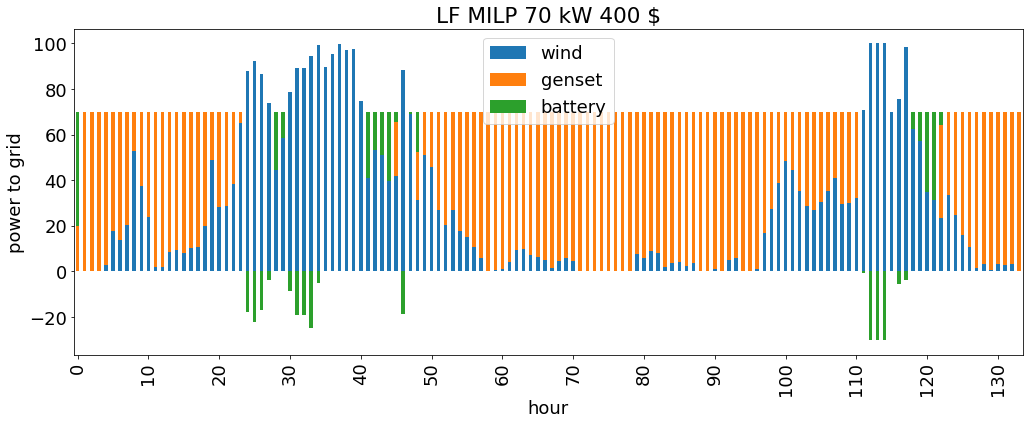
\includegraphics[scale=0.45]{/lf_70_400.png}
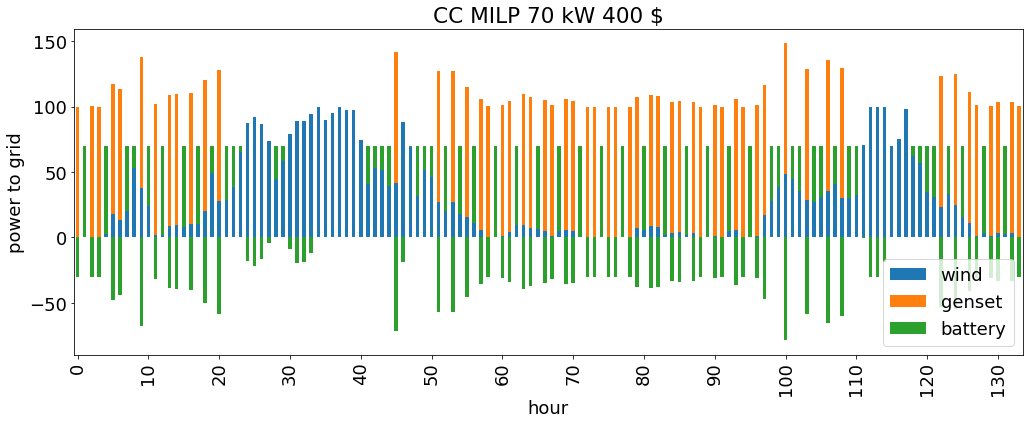
\includegraphics[scale=0.45]{/cc_70_400.png}
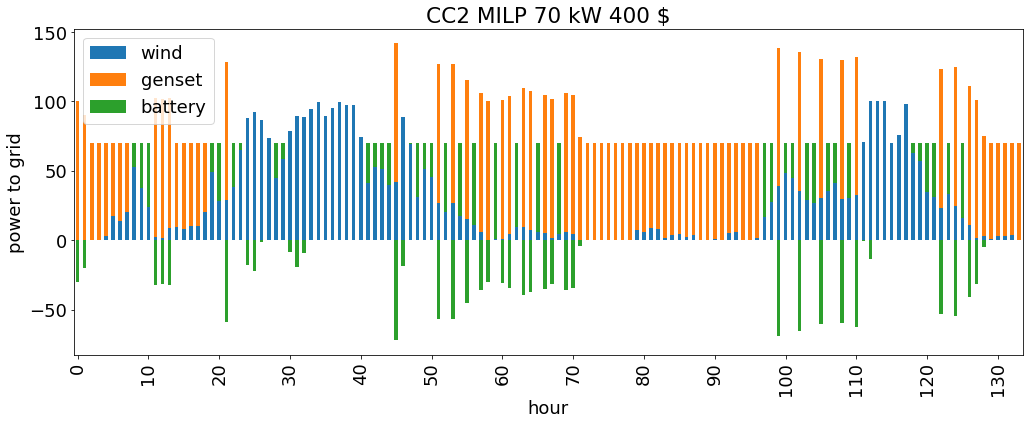
\includegraphics[scale=0.45]{/cc2_70_400.png}
\centering
\caption{Графики баланса мощности из численных экспериментов по сравнению стратегий планирования. Мощность нагрузки 70кВт, стоимость накопителя 1000\$/кВт ч. Положительные значения соответствуют генерации, отрицательные~---аккумуляции.}
\label{fig:res_70_400}
\end{figure}

\begin{figure}[H]
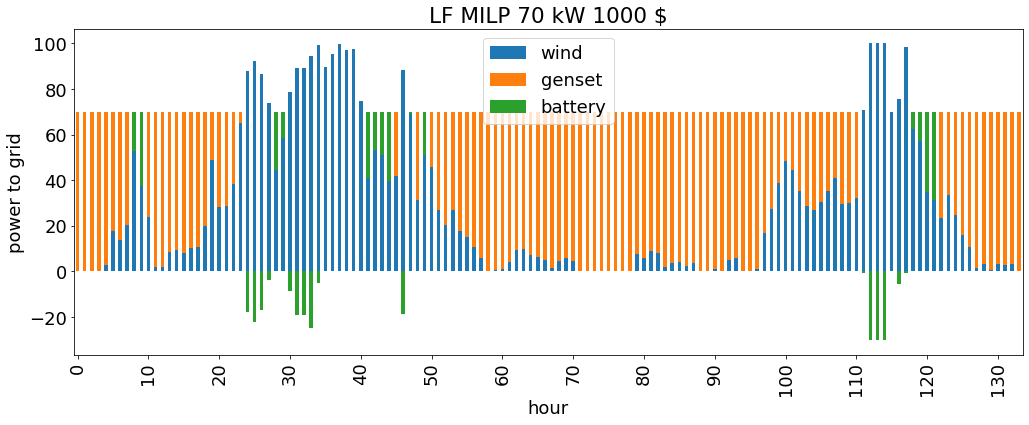
\includegraphics[scale=0.45]{/lf_70_1000.png}
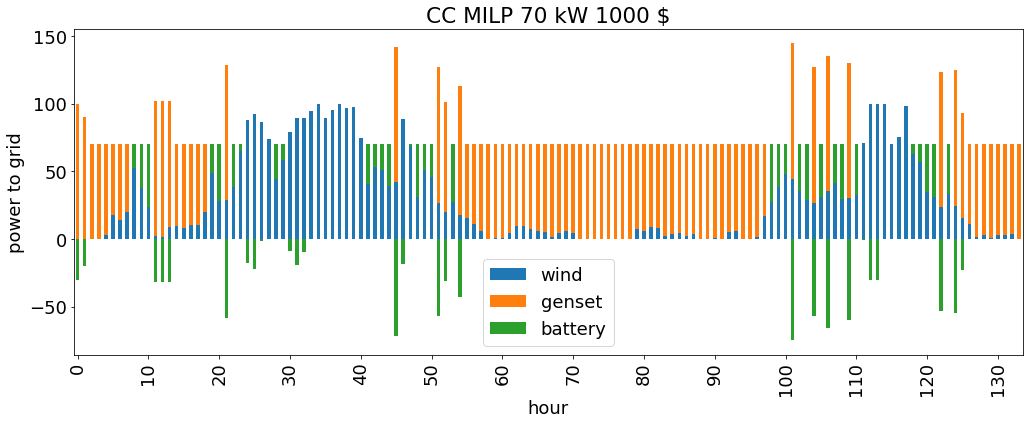
\includegraphics[scale=0.45]{/cc_70_1000.png}
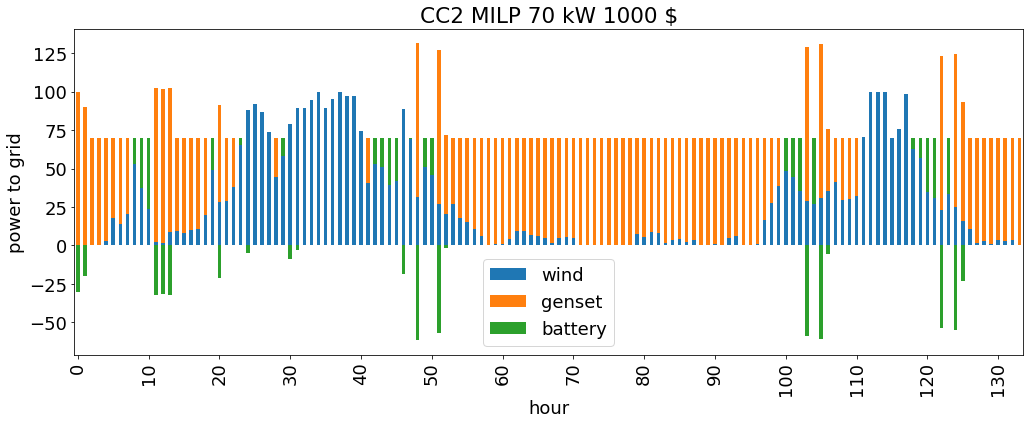
\includegraphics[scale=0.45]{/cc2_70_1000.png}
\caption{Графики баланса мощности из численных экспериментов по сравнению стратегий планирования. Мощность нагрузки 70кВт, стоимость накопителя 400\$/кВт ч. Положительные значения соответствуют генерации, отрицательные~---аккумуляции.}
\label{fig:res_70_1000}
\end{figure}

\begin{figure}[H]
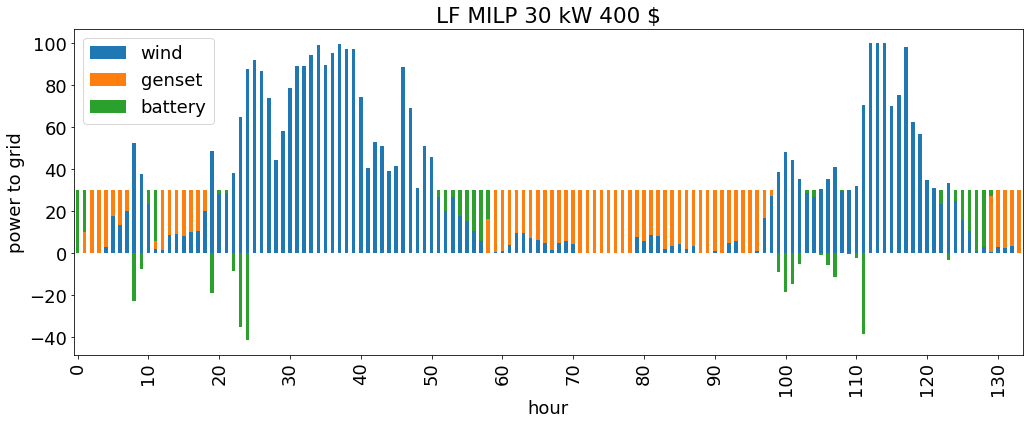
\includegraphics[scale=0.37]{/lf_30_400.png}
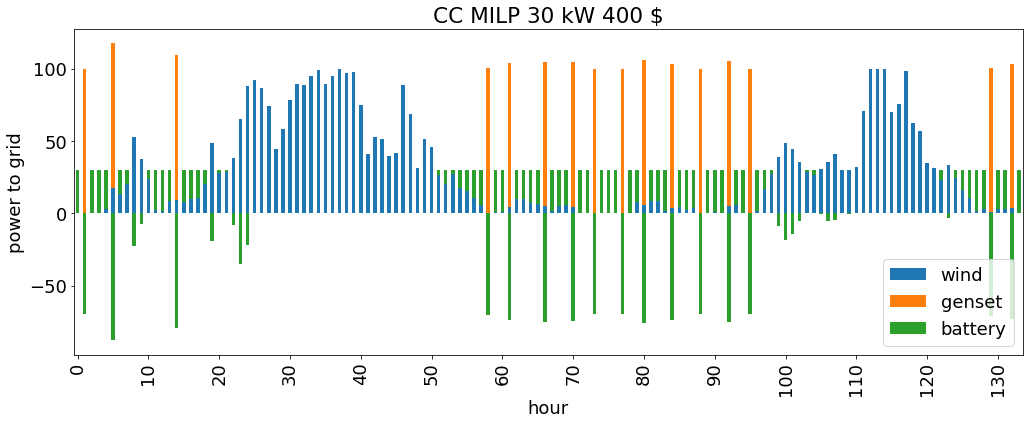
\includegraphics[scale=0.37]{/cc_30_400.png}
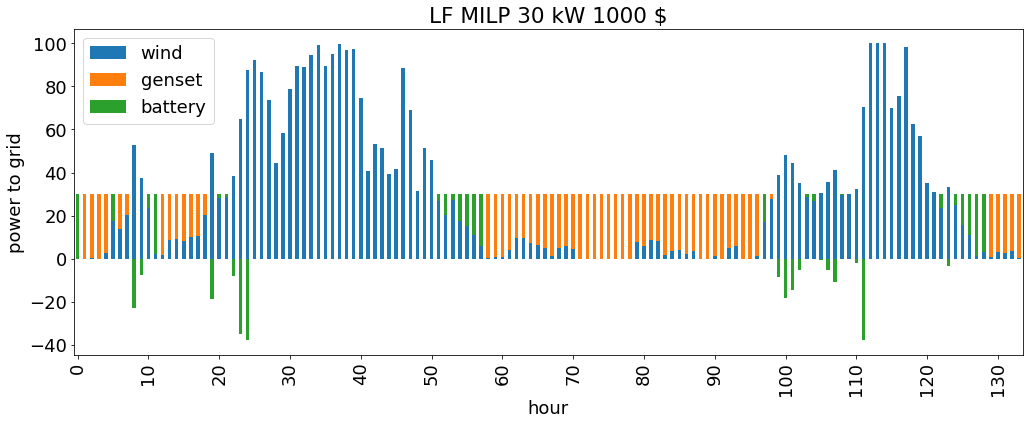
\includegraphics[scale=0.37]{/lf_30_1000.png}
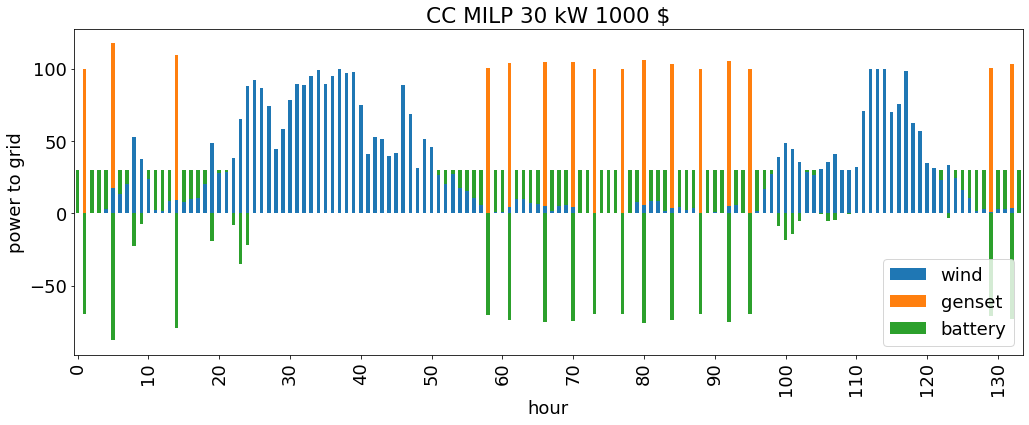
\includegraphics[scale=0.37]{/cc_30_1000.png}
\caption{Графики баланса мощности из численных экспериментов по сравнению стратегий планирования. Мощность нагрузки 70кВт. Положительные значения соответствуют генерации, отрицательные~---аккумуляции.}
\label{fig:res_30}
\end{figure}


\newpage
\printbibliography[heading=bibintoc, title={Список литературы}]

\end{document}
